\documentclass{article}

% COLM uses a format similar to ICLR.
% If you have the official colm2025_conference.sty, replace this preamble
% with \usepackage{colm2025_conference}.  The self-contained preamble below
% produces the same page geometry so the draft compiles out of the box.

% ---- packages ---------------------------------------------------------------
\usepackage[utf8]{inputenc}
\usepackage[T1]{fontenc}
\usepackage{amsmath,amssymb,amsfonts,amsthm}
\usepackage{mathtools}
\usepackage{bm}
\usepackage{bbm}
\usepackage{algorithm}
\usepackage{algorithmic}
\usepackage{booktabs}
\usepackage{graphicx}
\usepackage{hyperref}
\usepackage{url}
\usepackage{xcolor}
\usepackage[expansion=false]{microtype}
\usepackage{natbib}
\usepackage[margin=1in]{geometry}
\usepackage{enumitem}

% ---- notation shortcuts ------------------------------------------------------
\newcommand{\R}{\mathbb{R}}
\newcommand{\E}{\mathbb{E}}
\newcommand{\KL}{\mathrm{KL}}
\newcommand{\ot}{o_t}
\newcommand{\at}{a_t}
\newcommand{\rt}{r_t}
\newcommand{\zt}{z_t}
\newcommand{\dt}{d_t}
\newcommand{\hstate}{h_t}
\DeclareMathOperator{\softmax}{softmax}
\DeclareMathOperator{\SiLU}{SiLU}
\DeclareMathOperator{\RMSNorm}{RMSNorm}
\DeclareMathOperator{\symlog}{symlog}
\DeclareMathOperator{\diag}{diag}

% ==============================================================================
\title{Input-Affine Conditioning of Selective State-Space Models Is Gauge-Absorbable:\\A Mechanistic Null for FiLM-Style Regime Conditioning of Mamba}

\author{
  Anonymous Authors \\
  \texttt{anonymous@institution.edu}
}

\date{}

\begin{document}
\maketitle

% ==============================================================================
% ABSTRACT
% ==============================================================================
\begin{abstract}
Selective state-space models (Mamba) have reshaped long-context sequence
modeling, yet which forms of conditioning survive their training dynamics
is poorly understood.  We study FiLM-style regime conditioning of a Mamba
backbone---a per-block, channel-wise affine on each block's input, meant
to steer the input-dependent selective-scan parameters
$\Delta,\mathbf{B},\mathbf{C}$---and find it a \textbf{decisive null}:
under joint training the modulation collapses to identity and cannot be
forced active even by direct supervision.  We explain this
mechanistically.  An input-side affine is a \emph{gauge} direction that
folds losslessly into the block's own $\Delta/\mathbf{B}/\mathbf{C}$
projections, so the optimizer slides it back to identity.  The signature
is dataset- and architecture-invariant: forced-active, ER-supervised
escalations decay to identity with a shared time constant
($\tau\approx7000$ steps, $R^2>0.999$) across three very different
distributions---FI-2010 equities, Kaggle crypto spot books, and
Polymarket prediction markets---implicating the optimizer, not the data.
We then sharpen the mechanism with an output-side placement that gates
each block's output instead of its input.  Its multiplicative scale merely
folds into the block's \emph{other} (bias-free output) projection and
decays with the same constant ($\tau\approx7000$ on both datasets,
$R^2>0.999$), while the one genuinely non-absorbable component---an additive
shift---decays in lockstep.  The null is thus overdetermined: gauge
absorption removes every direction the host weights can represent, and
reconstruction dominance removes the one they cannot.  Escaping both would
require modulating the scan parameters \emph{inside} the fused kernel, which
our hardware cannot run.
The financial datasets are a demonstration substrate, not the subject; and
the same study yields a positive result the architecture did \emph{not}
carry.  Conditioning the dynamics did not help, but a
selective-participation \emph{strategy gate}---a decision rule, not an
architecture---turns the model's directionally informative settlement
signal into a survivable economic edge: in the high-predictability regime
the gate targets, a market-block bootstrap over $127$ independent held-out
markets gives $\mathrm{P(profit)}{=}1.0$, $95\%$ CI
$[{+}\$2{,}445,\,{+}\$7{,}747]$.  Crucially the edge is
\emph{architecture-independent}---a logistic regression on the same
features reproduces it---so the operative variable is the spot-conditioned
pipeline and the gate, not the sequence model.  Consistent with this, a
matched-parameter ablation (Mamba-1/2/3 and a Mamba-3-matched Transformer)
shows no backbone dominates: exactly what a result about how selective
scans \emph{train}, rather than which one is best, should predict.
\end{abstract}

% ==============================================================================
% 1  INTRODUCTION
% ==============================================================================
\section{Introduction}\label{sec:intro}

Modern limit order books generate high-frequency, high-dimensional tick
streams whose statistical properties shift with market regime---trending
versus mean-reverting phases, liquidity crises, and information
events---making them a demanding testbed for sequential world models.
Model-based reinforcement learning has shown that compact world models
can match or exceed much larger model-free agents in \emph{game}
environments~\citep{wang2024drama, hafner2023dreamerv3}, but these
systems have been developed almost exclusively on stationary domains
(Atari, DMC, MemoryMaze) where the observation distribution is fixed
after training.

Financial markets violate this stationarity assumption: the
data-generating process itself changes over time, driven by latent
regime shifts that alter volatility, liquidity, and the informational
content of order flow.  An agent trained on one regime may degrade when
the market transitions to another.  This failure mode motivates two
questions that guide the present work.  First, \emph{can a structured
state-space world model learn LOB dynamics offline?}  Second, and more
central, \emph{does explicit regime inference improve a world model's
behaviour under distributional shift relative to an unmodulated
backbone?}  The second question is the one our design is built to
answer.  We answer it \emph{negatively}: across every objective we test,
regime conditioning collapses to identity under joint training and does
not improve out-of-regime behaviour (Section~\ref{sec:results}).  That
negative redirected us to a third question the data made unavoidable:
\emph{if the model is shown the underlying spot path that defines
settlement, can its predictions be turned into profitable trades?}  They
can; and broader validation reveals a fourth: \emph{does supervising the
tradeable expected value directly, rather than the settlement probability,
eliminate the regime failure the settlement head hides at smaller scale?}
It does.

We adapt the Drama world-model framework~\citep{wang2024drama} to LOB
microstructure, taking the selective state-space sequence model at its
core---the same model family that has reshaped long-context sequence
modeling---and stress-testing it under genuine non-stationarity, where the
central question is not perplexity but \emph{which forms of conditioning a
selective scan's training dynamics will actually use}.  Our contributions
are organized around that question.

\paragraph{(1) A mechanistic null---and its boundary---for FiLM
conditioning of selective scans.}
Our central contribution is a sequence-modeling result.  We introduce a
\emph{RegimeFiLM} modulator that infers a categorical latent regime and
emits per-block, channel-wise affine parameters ($\gamma,\beta$); because
the selective-scan parameters $\Delta,\mathbf{B},\mathbf{C}$ are
input-dependent (Section~\ref{sec:ssm_prelim}), applying the affine to each
block's input is the natural way to push a regime signal \emph{into} the
state-space dynamics without touching the CUDA kernel.  Despite an exact
zero-initialized control and the strongest activation pressure we could
apply---forced-active initialization plus direct supervision of the
router---the modulation decays to identity on every objective and dataset
we test.  We explain it: an input-side affine is a \emph{gauge} direction
that folds losslessly into the block's own $\Delta/\mathbf{B}/\mathbf{C}$
projections, so joint training returns it to identity, with a dataset- and
architecture-invariant decay signature ($\tau\approx7000$, $R^2>0.999$;
Section~\ref{sec:results_null}).  An output-side placement sharpens
the mechanism rather than escaping it: the multiplicative scale folds into the
block's bias-free output projection and decays identically, while the
non-absorbable additive shift decays in lockstep, so the null is
\emph{overdetermined}---by gauge absorption and reconstruction dominance
together---and a surviving modulation would have to act inside the fused kernel
(Section~\ref{sec:results_null}).

\paragraph{(2) A world-model substrate across three LOB distributions, and
an architecture-agnosticism check.}
To stress the mechanism on genuinely different data, we build a Mamba-3
world model for LOB microstructure in the DreamerV3/Drama
lineage~\citep{hafner2023dreamerv3, wang2024drama, lahoti2026mamba3}: a
Transformer-over-depth encoder with binary-market invariants (boundary
distance, logit-space velocity, Amihud illiquidity, variance ratio), Lopez
de Prado bar aggregation, and direction/Hawkes/settlement auxiliary heads,
exercised on FI-2010 equities, Kaggle crypto spot books, and Polymarket
prediction markets.  The backbone is a substrate, not a claim: under
matched parameters \emph{no} backbone---Mamba-1, Mamba-2, Mamba-3 SISO, or
a Mamba-3-matched Transformer---dominates across datasets
(Section~\ref{sec:results_ablation}), exactly as a result about how
selective scans \emph{train}, rather than which one is best, should predict.

\paragraph{(3) What worked instead: a strategy gate and a direct-EV head.}
The same study yields a positive result the architecture did \emph{not}
carry.  Given the spot path that \emph{defines} settlement, the model's
directionally informative settlement probability---traded by a
selective-participation strategy that bets only when a causal
predictability gate fires---is a survivable, naive-beating economic edge,
placed away from zero by a market-block bootstrap over independent held-out
markets in the regime the gate targets
(Sections~\ref{sec:results_edge},~\ref{sec:pnl}).  The edge is
architecture-independent: a logistic regression on the same features
reproduces it (Section~\ref{sec:results_baseline}), so what carries it is
the spot-conditioned pipeline and the gate, not the sequence model.  A
\textbf{BookRelativeEdgeHead} that supervises the per-tick expected value
of each side net of the spread makes the low-predictability regime robust
where the raw settlement head is marginal (P(profit) $0.63\!\to\!0.99$;
regime spread $6.2{\times}$ smaller), at comparable total PnL
(Section~\ref{sec:results_ev}).  Conditioning the \emph{dynamics} did not
help; a decision rule over the model's outputs did---the same lesson the
null teaches, from the other side.

% ==============================================================================
% 2  RELATED WORK
% ==============================================================================
\section{Related Work}\label{sec:related}

\paragraph{World models and model-based RL.}
World models learn a compressed dynamics model of the environment and
use it to train a policy in imagination~\citep{ha2018world}.
DreamerV3~\citep{hafner2023dreamerv3} established the current template:
an RSSM with $32\!\times\!32$ categorical latents, symlog two-hot reward
decoding, and a single hyperparameter set across domains.
Drama~\citep{wang2024drama} replaced the RSSM's GRU with a Mamba-2
selective state-space model and reported a 105\% normalized score on
Atari100k with a 7M-parameter agent matching systems roughly $30\times$
larger.  TD-MPC2~\citep{hansen2024tdmpc2} pursues a decoder-free
trajectory-optimization alternative at 317M parameters.  FinMamba3
inherits the DreamerV3/Drama architecture, instantiates its dynamics with
a Mamba-3 selective state-space backbone, and adds explicit regime
conditioning, a capability we have not found in prior world models.

\paragraph{Structured state-space models and Mamba.}
Structured state-space models (S4, S5, Mamba) provide
$O(n)$-complexity alternatives to
Transformers~\citep{gu2022efficiently, smith2023s5, gu2024mamba}.
Mamba~\citep{gu2024mamba} introduced \emph{selective} state spaces in
which the discretization step $\Delta$ and input projection
$\mathbf{B}$ are input-dependent, enabling content-aware filtering.
Mamba-2~\citep{dao2024mamba2} formulated the duality between selective
state spaces and structured masked attention.
Mamba-3~\citep{lahoti2026mamba3} extends the selective SSM with
multi-input multi-output (MIMO) state transitions.  In financial time
series, MambaTS~\citep{mambats2024} applies Mamba to multivariate
forecasting, MambaStock~\citep{mambastock2024} to equity prediction, and
CryptoMamba~\citep{sepehri2025cryptomamba} to cryptocurrency price
prediction; none couples Mamba with a world-model POMDP formulation or
end-to-end regime inference.  We note that the name ``FinMamba'' has been
used for an unrelated Mamba-GNN stock-movement model; our system is
distinct in problem formulation (a generative LOB world model) and we
refer to it as FinMamba3 throughout.

\paragraph{Deep learning on limit order books.}
DeepLOB~\citep{zhang2019deeplob} established the CNN+LSTM architecture
for LOB mid-price direction prediction on the FI-2010
benchmark~\citep{ntakaris2018benchmark}.  Subsequent work introduced
Transformer attention: TLOB~\citep{berti2025tlob} uses a dual
spatial/temporal attention mechanism that captures cross-level
dependencies in LOB snapshots and reports improved generalization under
volatile conditions, while HLOB~\citep{hlob2024} introduces
persistence-aware blocks grounded in information-filtering networks.
The LOBFrame codebase~\citep{lobframe2024} provides a canonical
evaluation protocol and reports that high forecasting accuracy does not
necessarily translate into actionable trading signals.  All of these are
\emph{discriminative} models: they map observed LOB features to a label
or regression target, and none learns a generative dynamics model usable
for latent-space planning or imagination-based RL.

\paragraph{Generative models of LOB dynamics.}
A parallel line of work models LOB microstructure generatively.
\citet{nagy2023lobs5} propose LOBS5, an autoregressive token-level
generative model of Level-3 message flow built on a deep state-space
network, evaluated under the LOB-Bench
framework~\citep{nagy2025lobbench}.
\citet{backhouse2025painting} apply spatio-temporal diffusion models to
Level-2 snapshots and report strong stylized-fact fidelity on LOB-Bench.
These works share our goal of modelling LOB dynamics generatively but
differ from FinMamba3 in three respects: (i)~they target simulation
fidelity (reproducing stylized facts) rather than a compact latent
representation for control; (ii)~they do not learn a POMDP world model
with a prior usable for policy imagination; and (iii)~neither conditions
its dynamics on an inferred latent regime.  These are complementary
approaches rather than direct baselines for the world-model objective.

\paragraph{Regime-switching and non-stationarity in financial ML.}
Classical regime-switching models (Hamilton HMM, Markov-switching GARCH)
identify discrete market states from price
processes~\citep{hamilton1989new}.  Modern approaches either use
changepoint detection as a preprocessing step, including Bayesian online
methods~\citep{adams2007bayesian}, or learn regime embeddings
end-to-end~\citep{lim2021time}.  FiLM
conditioning~\citep{perez2018film} has been applied in vision and
multi-task settings to inject context into learned representations, but
we are not aware of prior work applying FiLM to modulate state-space
dynamics in a financial world model.

\paragraph{Scale redundancy and scale-invariance.}
That a channel-wise affine placed before a linear map is redundant with that
map is a known theme in the normalization literature.
\citet{vanlaarhoven2017l2} shows that weights feeding a normalization layer are
scale-invariant, so $L_2$ regularization acts on their \emph{scale}---and thus
the effective learning rate---rather than as a capacity control;
\citet{hoffer2018norm} and \citet{li2020exp} build on the same scale-invariance
to re-derive weight decay as an effective-learning-rate schedule.  Our null is
an instance of this redundancy, but in a setting it has not been analyzed: the
absorbed affine is not a static normalization gain but a per-regime,
\emph{input-dependent} FiLM, and it folds into the selective scan's own
$W_\Delta/W_B/W_C$ projections.  What is new here is therefore (i) the
input-dependent selective-scan instantiation; (ii) the dataset- and
architecture-invariant decay signature ($\tau\approx7000$, $R^2>0.999$) that
attributes the collapse to the optimizer; (iii) the output-side placement
showing the null is \emph{overdetermined} (gauge absorption plus reconstruction
dominance); and (iv) the practical consequence that the only kernel-friendly,
drop-in form of regime conditioning is exactly the absorbable one---so the
redundancy is the default a practitioner reaches for, not a corner case.

\paragraph{Prediction-market microstructure.}
Polymarket is a decentralized prediction market in which binary-outcome
contracts trade on a central-limit order book.  Effective spreads on
these contracts are wide relative to equity LOBs, so per-tick mid-price
changes are dominated by spread-bouncing noise rather than information;
this motivates our use of Lopez de Prado bar
aggregation~\citep{deprado2018advances} for tick-stream denoising.

% ==============================================================================
% 3  PRELIMINARIES
% ==============================================================================
\section{Preliminaries}\label{sec:prelim}

\subsection{Partially Observable Markov Decision Processes}

We model the LOB trading environment as a POMDP
$(\mathcal{S}, \mathcal{A}, \mathcal{O}, T, O, R, \gamma)$ where
$\mathcal{S}$ is the latent state space (the full microstructure state,
including hidden liquidity, informed-trader intent, and regime),
$\mathcal{A}$ the discrete action space,
$\mathcal{O}$ the observation space (the visible LOB snapshot),
$T(s'\mid s, a)$ the transition kernel,
$O(o \mid s)$ the observation model,
$R(s, a)$ the reward, and $\gamma$ the discount.  At each tick~$t$ the
agent observes $\ot \in \R^F$ (an $F$-dimensional feature vector
extracted from the LOB), selects $\at \in \mathcal{A}$, and receives
$\rt$.  The true state~$s_t$ is never observed.

\subsection{World-Model Architecture (DreamerV3 / Drama)}

A world model approximates the POMDP by learning four components from
offline trajectories $\{(\ot, \at, \rt)\}_{t=1}^{T}$.

\paragraph{Encoder.}
A function $\mathrm{enc}_\phi: \mathcal{O} \to \R^{d_e}$ mapping the raw
observation to a compact embedding $e_t = \mathrm{enc}_\phi(\ot)$.

\paragraph{Posterior (representation model).}
A categorical distribution
$q_\phi(\zt \mid e_t, \hstate) = \mathrm{Cat}(\zt; \bm{\pi}^{\text{post}}_t)$
over the discrete latent $\zt \in \{0,1\}^{C \times D}$, parameterized
as a $C \times D$ one-hot categorical (we use $C = D = 16$, yielding a
256-dimensional flattened sample).  Samples use the straight-through
Gumbel estimator.

\paragraph{Sequence model (dynamics prior).}
A recurrence that compresses past latents and actions into a
deterministic hidden state,
\begin{equation}\label{eq:sequence_model}
  \hstate = f_\theta(\zt, \at, h_{t-1}),
\end{equation}
from which a prior $p_\theta(\zt \mid \hstate) = \mathrm{Cat}(\zt;
\bm{\pi}^{\text{prior}}_t)$ is predicted.  In DreamerV3 this recurrence
is a GRU; in Drama it is a Mamba-2 selective state-space layer; in
FinMamba3 it is a stack of Mamba-3 blocks
(Section~\ref{sec:mamba3}).

\paragraph{Decoder and auxiliary heads.}
An observation decoder $\hat{o}_t = \mathrm{dec}_\theta(\zt)$
reconstructs the input; optional reward and termination heads predict
$\hat{r}_t$ and $\hat{\delta}_t$.

\paragraph{Training objective.}
The world model is trained by minimizing
\begin{equation}\label{eq:world_model_loss}
  \mathcal{L}_{\text{wm}}
  = \underbrace{\mathcal{L}_{\text{recon}}}_{\text{observation}}
  + \underbrace{\mathcal{L}_{\text{dyn}}}_{\text{dynamics KL}}
  + \beta\,\underbrace{\mathcal{L}_{\text{rep}}}_{\text{representation KL}}
  + \sum_k \lambda_k \mathcal{L}_k^{\text{aux}},
\end{equation}
where $\mathcal{L}_{\text{recon}}$ is the reconstruction loss (MSE or
Student-$t$ negative log-likelihood),
$\mathcal{L}_{\text{dyn}} = \KL[q_\phi(\zt \mid e_t, \hstate)\,\|\,
\mathrm{sg}[p_\theta(\zt \mid \hstate)]]$ trains the prior to match the
posterior (with the posterior stopped-gradient),
$\mathcal{L}_{\text{rep}} = \KL[\mathrm{sg}[q_\phi]\,\|\,p_\theta]$
pulls the posterior toward the prior, and both KL terms use a free-bits
floor of 1.0~nat per step to prevent degenerate posterior--prior
collapse~\citep{hafner2023dreamerv3}.

\subsection{Selective State-Space Models}\label{sec:ssm_prelim}

A linear time-invariant (LTI) state-space model maps an input sequence
$x(t) \in \R^{d}$ to an output $y(t) \in \R^{d}$ via a latent state
$h(t) \in \R^{N}$:
\begin{equation}\label{eq:continuous_ssm}
  \dot{h}(t) = \mathbf{A}\,h(t) + \mathbf{B}\,x(t), \qquad
  y(t) = \mathbf{C}\,h(t),
\end{equation}
with $\mathbf{A} \in \R^{N \times N}$,
$\mathbf{B} \in \R^{N \times d}$,
$\mathbf{C} \in \R^{d \times N}$.
After zero-order-hold discretization with step $\Delta$,
\begin{equation}\label{eq:discrete_ssm}
  h_t = \bar{\mathbf{A}}\,h_{t-1} + \bar{\mathbf{B}}\,x_t, \qquad
  y_t = \mathbf{C}\,h_t,
\end{equation}
where $\bar{\mathbf{A}} = \exp(\Delta\,\mathbf{A})$ and
$\bar{\mathbf{B}} = (\Delta\,\mathbf{A})^{-1}
(\bar{\mathbf{A}} - \mathbf{I})\,\Delta\,\mathbf{B}$.

\paragraph{Mamba (selective SSM).}
Mamba~\citep{gu2024mamba} makes $\Delta_t$, $\mathbf{B}_t$, and
$\mathbf{C}_t$ \emph{input-dependent} via learned linear projections of
$x_t$, breaking the LTI assumption and enabling content-aware gating.
This \emph{selection mechanism} is the property we exploit: because
$\Delta_t = \softmax(W_\Delta\,x_t)$, $\mathbf{B}_t = W_B\,x_t$, and
$\mathbf{C}_t = W_C\,x_t$, any affine transformation of $x_t$ propagates
directly into all three scan parameters.

\paragraph{Mamba-3.}
Mamba-3~\citep{lahoti2026mamba3} extends the selective SSM with
multi-input multi-output (MIMO) state transitions that couple
information across heads within each layer.  It also incorporates rotary
position embeddings (RoPE) on a configurable fraction of the head
dimension and an optional output-projection normalization.  We
instantiate the single-input single-output (SISO) configuration
throughout; the MIMO configuration is not evaluated in this work.

% ==============================================================================
% 4  METHODOLOGY
% ==============================================================================
\section{Methodology}\label{sec:method}

FinMamba3 adapts the Drama world-model framework to LOB microstructure
along four axes: the observation encoder
(Section~\ref{sec:lob_encoder}), the sequence backbone
(Section~\ref{sec:mamba3}), the regime-modulated dynamics
(Section~\ref{sec:regime_film}), and the auxiliary training objectives
(Section~\ref{sec:aux_heads}).

% --------------------------------------------------------------------------
\subsection{Transformer-over-Depth LOB Encoder}\label{sec:lob_encoder}

Raw LOB snapshots are represented as a flat feature vector
$\ot \in \R^F$ with $F = K \cdot F_{\ell} + F_{\tau}$.  We use
$K = 10$ depth levels, each carrying $F_{\ell} = 8$ per-level features
(relative price, log size, log cumulative depth, volume share, price
gap, level index, side indicator, log staleness), and
$F_{\tau} = 20$ tick-level aggregate features (midprice, spread,
imbalance, microprice, order-flow imbalance, trade intensity, rolling
volatility, plus six binary-market invariants described below).

Rather than flattening the $K$ depth levels and applying an MLP---which
discards the ordering and cross-level structure of the book---we treat
each level as a token and apply a Transformer encoder over depth:
\begin{equation}\label{eq:lob_enc}
  \mathrm{tok}_k = W_{\ell}\,\ot^{(k)} + \mathrm{pos}_k,
  \qquad k = 1, \ldots, K,
\end{equation}
where $\ot^{(k)} \in \R^{F_\ell}$ is the $k$-th level's feature vector,
$W_\ell \in \R^{d_m \times F_\ell}$ is a shared linear projection, and
$\mathrm{pos}_k \in \R^{d_m}$ is a learned positional embedding.  A
\textsc{[CLS]} token initialized with the tick-level features
$\ot^{(\tau)}$ via a two-layer MLP is prepended.  The full sequence
$[\textsc{CLS};\,\mathrm{tok}_1;\,\ldots;\,\mathrm{tok}_K]$ is processed
by a $2$-layer, $4$-head pre-norm Transformer encoder with GELU
activation and $d_m = 128$.  The output at the \textsc{[CLS]} position
is projected to a $d_e = 1024$-dimensional embedding:
\begin{equation}
  e_t = W_{\text{out}}\,\RMSNorm\bigl(\mathrm{TF}([\textsc{CLS};\,
  \mathrm{tok}_1;\,\ldots;\,\mathrm{tok}_K])_0\bigr).
\end{equation}
This design preserves the depth ordering of the book, lets attention
capture cross-level dependencies (bid--ask symmetry, depth-curve shape),
and accommodates different numbers of levels.  The codebase provides a
flat-MLP encoder for a controlled comparison; we do not run that ablation in
this paper (Appendix~\ref{app:unevaluated}) and make no superiority claim.

\paragraph{Binary-market features.}
Polymarket contracts are binary outcomes whose prices are bounded
probabilities in $[0, 1]$.  Liquidity and information dynamics change
qualitatively near the probability boundaries and are sensitive to
time-to-expiry.  We append six tick-level features that capture these
invariants:
\begin{itemize}[nosep]
  \item \emph{Boundary distance}: $\min(m_t,\; 1 - m_t)$, where $m_t$
    is the midprice.
  \item \emph{Boundary-scaled depth}: $\log(\text{depth}) \cdot
    \min(m_t, 1 - m_t)$.
  \item \emph{Logit-mid velocity and acceleration}: first and second
    differences of $\mathrm{logit}(m_t)$, the natural unbounded
    coordinate for an implied probability.
  \item \emph{Amihud illiquidity}~\citep{amihud2002illiquidity}:
    rolling $|\text{logit return}| / \text{depth}$.
  \item \emph{Variance ratio}: Lo--MacKinlay $\mathrm{VR}(2)$ of logit
    returns; values below~1 indicate mean reversion, above~1 trending.
\end{itemize}
These are appended (not interleaved) to preserve backward compatibility
with existing feature indices.  For the FI-2010 benchmark, binary-market
features are omitted ($F_\tau = 14$, $F = 94$).

\paragraph{Bar aggregation.}
Because raw per-tick midprice changes on wide-spread contracts are
dominated by spread-bouncing noise, we implement five Lopez de Prado bar
types~\citep{deprado2018advances}---time, volume, dollar,
tick-imbalance, and CUSUM---each producing the same $F$-dimensional
feature vector so the downstream pipeline is aggregation-agnostic.

% --------------------------------------------------------------------------
\subsection{Mamba-3 Sequence Backbone}\label{sec:mamba3}

The posterior latent samples $\zt \in \R^{256}$ (from the
$16\!\times\!16$ categorical) are fed through a stem network
\begin{equation}
  x_t^{(0)} = \SiLU\!\bigl(\RMSNorm(W_s\,\zt)\bigr) \in \R^{d_h},
\end{equation}
with $d_h = 512$, followed by an $L$-layer ($L = 4$) stack of Mamba-3
blocks.  Each block applies a pre-norm residual,
\begin{equation}\label{eq:mamba_block}
  x_t^{(\ell)} = x_t^{(\ell-1)} + \mathrm{Mamba3}\!\bigl(
  \RMSNorm(x_t^{(\ell-1)})\bigr),
  \qquad \ell = 1, \ldots, L.
\end{equation}
The Mamba-3 block parameterizes a selective state-space model in its
single-input single-output (SISO) configuration with
$d_{\text{state}} = 128$, head dimension 64 (8 heads for $d_h = 512$),
chunk size~16, and RoPE on 50\% of the head dimension.  The
final hidden state is $\hstate = \RMSNorm(x_t^{(L)}) \in \R^{d_h}$.

We provide matched YAML
configurations for Mamba-1, Mamba-2, Mamba-3 SISO, and a Transformer
backbone so that the architecture ablation can be reproduced with a
single command per variant.

% --------------------------------------------------------------------------
\subsection{Regime-Aware FiLM Modulation}\label{sec:regime_film}

A world model trained on one regime may produce inaccurate rollouts in
another.  We condition the Mamba dynamics on an inferred latent regime.

\paragraph{Design constraint.}
The Mamba-3 blocks are provided by the upstream \texttt{mamba-ssm}
library and execute fused CUDA/TileLang kernels.  Modifying $\Delta_t$,
$\mathbf{B}_t$, or $\mathbf{C}_t$ inside the kernel would be fragile and
would invalidate prebuilt GPU wheels.

\paragraph{Key idea.}
Because $\Delta_t$, $\mathbf{B}_t$, and $\mathbf{C}_t$ are
input-dependent functions of each block's input
(Section~\ref{sec:ssm_prelim}), a channel-wise affine transformation of
the block input propagates the regime signal \emph{into the
selective-scan parameters through the selection mechanism itself},
without touching the kernel.

\paragraph{RegimeFiLM modulator.}
Let $x_t^{(0)}$ denote the stem output.  A \emph{regime head}---a linear
projection followed by a softmax over $R = 8$ regimes---infers a soft
categorical distribution and produces a regime embedding via a weighted
combination of a learned embedding table:
\begin{equation}\label{eq:regime_head}
  \bm{\alpha}_t = \softmax(W_r\,x_t^{(0)}) \in \R^R,
  \qquad
  r_t = \bm{\alpha}_t^\top E \in \R^{d_r},
\end{equation}
where $E \in \R^{R \times d_r}$ with $d_r = 32$.  A hypernetwork maps
$r_t$ to per-block FiLM parameters:
\begin{equation}\label{eq:film}
  [\tilde{\gamma}^{(1)}, \ldots, \tilde{\gamma}^{(L)},\;
   \tilde{\beta}^{(1)}, \ldots, \tilde{\beta}^{(L)}]
  = W_{\text{hyper}}\,r_t,
\end{equation}
with $W_{\text{hyper}} \in \R^{2Ld_h \times d_r}$.  Because $r_t$ is
low-dimensional ($d_r = 32$) while the FiLM output spans $2Ld_h$
channels, the modulation is deliberately low-rank in regime space: it
applies a small number of regime-specific affine directions rather than
arbitrary per-channel control.  We treat this bottleneck as a design
choice and report its sensitivity in the ablation.  The affine
parameters are bounded via $\tanh$ for bf16 stability,
\begin{equation}\label{eq:film_bounded}
  \gamma^{(\ell)} = 1 + \tanh(\tilde{\gamma}^{(\ell)}),
  \qquad
  \beta^{(\ell)} = \tanh(\tilde{\beta}^{(\ell)}),
\end{equation}
so that $\gamma^{(\ell)} \in (0, 2)$ and $\beta^{(\ell)} \in (-1, 1)$.
The Mamba block from Eq.~\eqref{eq:mamba_block} becomes
\begin{equation}\label{eq:mamba_film}
  x_t^{(\ell)} = x_t^{(\ell-1)}
  + \mathrm{Mamba3}\!\bigl(
    \gamma^{(\ell)} \odot \RMSNorm(x_t^{(\ell-1)})
    + \beta^{(\ell)}
  \bigr).
\end{equation}
Because the Mamba-3 block computes $\Delta_t =
\sigma(W_\Delta\,\tilde{x}_t)$, $\mathbf{B}_t = W_B\,\tilde{x}_t$,
$\mathbf{C}_t = W_C\,\tilde{x}_t$ from its input $\tilde{x}_t$, setting
$\tilde{x}_t = \gamma^{(\ell)} \odot \hat{x}_t + \beta^{(\ell)}$ makes
the scan parameters a function of both the observation and the inferred
regime.

\paragraph{Application site: input-affine vs.\ post-scan.}
Equation~\eqref{eq:mamba_film} applies the affine to the block \emph{input},
the form that routes the regime into $\Delta_t,\mathbf{B}_t,\mathbf{C}_t$
through the selection mechanism.  As a control (Section~\ref{sec:results_null})
we also expose a \emph{post-scan} site that gates the block \emph{output}
instead,
\begin{equation}\label{eq:mamba_film_postscan}
  x_t^{(\ell)} = x_t^{(\ell-1)}
  + \gamma^{(\ell)} \odot \mathrm{Mamba3}\!\bigl(\RMSNorm(x_t^{(\ell-1)})\bigr)
  + \beta^{(\ell)} .
\end{equation}
The two share the identical modulator (Eqs.~\eqref{eq:regime_head}--\eqref{eq:film_bounded});
only the application site differs.  This isolates the role of gauge structure:
the input-affine scale folds into the input projections $W_\Delta/W_B/W_C$,
while the post-scan scale folds into the bias-free output projection
$W_{\text{out}}$; only the post-scan additive shift is non-absorbable
(Section~\ref{sec:results_null}).

\paragraph{Initialization.}
The hypernetwork weights and biases are initialized to zero, so at the
start of training $\gamma^{(\ell)} = \mathbf{1}$ and
$\beta^{(\ell)} = \mathbf{0}$ for all~$\ell$.  This makes the modulated
backbone exactly identical to the unmodulated baseline at
initialization, providing a clean control and a stable warm-start.

\paragraph{Load-balancing regularizer.}
To discourage regime collapse (all timesteps assigned to one regime), we
add a Switch-Transformer-style
regularizer~\citep{fedus2022switch} that maximizes the entropy of the
batch-averaged regime distribution,
\begin{equation}\label{eq:load_balance}
  \mathcal{L}_{\text{regime}} = \lambda_{\text{ent}}
  \Bigl(\log R - H\!\bigl[\bar{\bm{\alpha}}\bigr]\Bigr),
  \qquad
  \bar{\bm{\alpha}} = \frac{1}{BL}\sum_{b,t} \bm{\alpha}_{b,t},
\end{equation}
where $H[\cdot]$ is the Shannon entropy, $B$ and $L$ are the batch size
and sequence length, and $\lambda_{\text{ent}} = 0.01$.  This
regularizes the \emph{marginal} regime usage while leaving per-step
assignments free to be peaky.

% --------------------------------------------------------------------------
\subsection{Episodic Memory}\label{sec:episodic_memory}

The Mamba hidden state provides parametric memory but is fixed after
training.  Under distributional shift at test time---rare patterns,
regime changes, or under-represented local behaviors---the parametric
model may fail to recognize them.

We augment the world model with a lightweight, CPU-side episodic memory
buffer that stores past hidden states and retrieves the $k$ nearest
neighbors (by cosine similarity) at each training step.  The retrieved
context is fused with the current hidden state via a gated residual,
\begin{equation}\label{eq:em_fusion}
  \tilde{h}_t = h_t + \sigma(W_g[h_t; m_t]) \odot \tanh(W_p[h_t; m_t]),
\end{equation}
where $m_t = \sum_{i=1}^{k} w_i\,v_i$ is the soft-attention-weighted
retrieval ($w_i$ from the cosine-similarity softmax, $v_i$ the stored
hidden states), and $\sigma$ is the sigmoid gate.

Two write policies are supported:
(i)~\emph{FIFO}: every last-frame hidden state is appended, oldest
evicted;
(ii)~\emph{Novelty-filtered}: only entries whose symmetric KL between
posterior and prior exceeds a threshold are written, so the buffer
becomes a catalog of regime-surprising states rather than a sliding
window of recent observations.  Whether episodic memory helps at
inference, and which write policy is preferable, is an open question we do
not resolve here: the module is implemented but its ablation is unevaluated
in this paper (Appendix~\ref{app:unevaluated}).

% --------------------------------------------------------------------------
\subsection{Observation Decoder and Reconstruction Loss}\label{sec:decoder}

The observation decoder maps the flattened latent sample
$\zt \in \R^{256}$ back to the flat LOB feature vector
$\hat{o}_t \in \R^F$ through a 3-layer MLP with RMSNorm and SiLU
activations.

Two decoder variants are provided.  The default uses a weighted MSE loss
in which size/flow features receive $2\times$ the weight of price
features:
\begin{equation}\label{eq:recon_mse}
  \mathcal{L}_{\text{recon}} = \frac{1}{BLF}
  \sum_{b,t,f} w_f\,(\hat{o}_{b,t,f} - o_{b,t,f})^2.
\end{equation}
The $2\times$ weighting is an empirical design choice motivated by the
observation that order-flow quantities carry directional information in
LOBs~\citep{cont2014price}; we do not claim the specific ratio is
optimal and treat it as a tunable hyperparameter.  The alternative is a
Student-$t$ negative log-likelihood decoder that predicts per-feature
mean $\mu_{t,f}$ and log-scale $\log\sigma_{t,f}$ with learnable degrees
of freedom~$\nu_f$:
\begin{equation}\label{eq:recon_studentt}
  \mathcal{L}_{\text{recon}}^{\text{St}} = -\frac{1}{BLF}
  \sum_{b,t,f} w_f \log p_{\text{St}}(o_{b,t,f};\,
  \mu_{b,t,f},\,\sigma_{b,t,f},\,\nu_f).
\end{equation}
The heavy-tailed Student-$t$ likelihood is intended to model the excess
kurtosis of LOB returns arising from discretized prices and occasional
regime jumps.

% --------------------------------------------------------------------------
\subsection{Auxiliary Heads}\label{sec:aux_heads}

Three domain-specific auxiliary heads inject microstructure inductive
bias into the world-model latent, each gated by a configuration flag and
contributing zero loss when its required labels are absent.

\paragraph{Direction head.}
A two-layer MLP predicts the three-class next-tick midprice direction
(down / flat / up) from the conditioned hidden state $\tilde{h}_t$,
trained with cross-entropy.  The direction threshold $\epsilon$ that
defines the flat bucket can be swept as a hyperparameter; a
multi-threshold variant averages the cross-entropy across a list of
thresholds so accuracy can be reported as a curve rather than a single
number:
\begin{equation}
  \mathcal{L}_{\text{dir}} = \frac{1}{|\mathcal{E}|}
  \sum_{\epsilon \in \mathcal{E}}
  \mathrm{CE}\!\bigl(\hat{y}_t,\; \mathrm{bucket}(\Delta m_t, \epsilon)\bigr).
\end{equation}

\paragraph{Hawkes intensity head.}
An MLP predicting log-intensity for buy and sell event arrivals, trained
with Poisson negative log-likelihood on observed event counts in a
forward window:
\begin{equation}
  \mathcal{L}_{\text{Hawkes}} = \sum_{s \in \{\text{buy},\text{sell}\}}
  \bigl[\hat{\lambda}_{t,s} - n_{t,s}\,\log\hat{\lambda}_{t,s}\bigr],
\end{equation}
where $\hat{\lambda}_{t,s} = \exp(\text{MLP}(\tilde{h}_t))_s$ and
$n_{t,s}$ is the observed count.  This head provides an order-arrival
self-supervised signal.

\paragraph{Settlement head.}
A binary classifier predicting the contract outcome (YES/NO) from the
latent, trained with binary cross-entropy optionally weighted by
closeness to expiry so the training pressure ramps up near resolution:
\begin{equation}
  \mathcal{L}_{\text{settle}} = -\bigl[(1 - \tau_t)\,
  y\log\hat{p}_t + (1 - y)\log(1 - \hat{p}_t)\bigr],
\end{equation}
where $\tau_t \in [0, 1]$ is the time-to-expiry fraction (1 at the
start, 0 at expiry) and $y \in \{0, 1\}$ is the binary outcome.  This
encourages the latent to encode information relevant to the terminal
payoff rather than only locally reconstructive features.

\paragraph{Book-relative EV head.}
A two-output MLP on the deterministic state $\hstate$ directly predicts
the per-tick expected value of buying each side of the book:
\[
  (\hat{e}_{\text{yes},t},\, \hat{e}_{\text{no},t})
  = \text{Linear}\!\bigl(\text{SiLU}(\text{Linear}(\hstate))\bigr),
\]
trained with Huber loss ($\delta=1$) against realized targets
\[
  e_{\text{yes}} = \text{outcome} - \text{ask}_{\text{yes}}, \qquad
  e_{\text{no}} = (1-\text{outcome}) - \text{ask}_{\text{no}},
\]
masking ticks where either ask is absent (zero book depth).  Unlike the
settlement head, when the book is efficiently priced the training target
is near zero and the strategy abstains; when the ask undershoots the
outcome the target is positive and a trade fires.  The trading rule is:
$\hat{e}_{\text{yes}} \geq \tau_e \wedge \hat{e}_{\text{yes}} >
\hat{e}_{\text{no}}$ triggers a BUY-YES order; symmetrically for
BUY-NO; otherwise abstain.

% --------------------------------------------------------------------------
\subsection{Full Training Objective}\label{sec:full_loss}

Combining all components, the FinMamba3 world-model loss is
\begin{equation}\label{eq:full_loss}
  \mathcal{L} =
  \mathcal{L}_{\text{recon}}
  + \mathcal{L}_{\text{dyn}}
  + \beta\,\mathcal{L}_{\text{rep}}
  + \lambda_{\text{dir}}\,\mathcal{L}_{\text{dir}}
  + \lambda_{\text{H}}\,\mathcal{L}_{\text{Hawkes}}
  + \lambda_{\text{S}}\,\mathcal{L}_{\text{settle}}
  + \lambda_{\text{EV}}\,\mathcal{L}_{\text{EV}}
  + \lambda_{\text{ent}}\,\mathcal{L}_{\text{regime}},
\end{equation}
where $\mathcal{L}_{\text{EV}} = \text{Huber}(\hat{e}_{\text{yes}},
e_{\text{yes}}) + \text{Huber}(\hat{e}_{\text{no}}, e_{\text{no}})$
is the book-relative EV loss (zero when the head is disabled),
with $\beta = 0.1$, $\lambda_{\text{dir}} = 0.5$,
$\lambda_{\text{H}} = 0.1$, $\lambda_{\text{S}} = 0.25$,
$\lambda_{\text{EV}} = 1.0$, and $\lambda_{\text{ent}} = 0.01$.  Reward and termination heads are gated
off during Phase~A pretraining (no reward signal in the offline buffer)
and enabled in Phase~B imagination-based RL, where the full
DreamerV3/Drama actor--critic loop applies.

The model is optimized with
LaProp~\citep{ziyin2021laprop} (learning rate $4 \times 10^{-5}$,
$\epsilon = 10^{-20}$, weight decay $10^{-4}$) with 500-step linear
warmup and cosine annealing over 15\,000 steps.  Gradient norms are
clipped at 100.  Mixed-precision (bf16) autocast is used with a NaN-guard
that skips the first 50 non-finite backward passes to absorb
selective-scan instabilities during early training.

% --------------------------------------------------------------------------
\subsection{Spot-Conditioned Polymarket Pipeline}\label{sec:spot_pipeline}

The settlement of a Polymarket binary contract is decided by the
\emph{underlying} spot price (the Chainlink/Binance close versus the open
reference), yet a pipeline that feeds the model only the contract's own
order book hides the variable that defines its label.  We rebuild the
Polymarket feature pipeline along five axes.
\emph{(i)~Spot path.}  Each tick carries the asset's spot log-return
since the market's open reference, its rolling realized volatility, and
the signed distance $(s_t - s_0)/s_0$ to the open.
\emph{(ii)~Time-to-expiry clock.}  Each tick carries
$\tau_t = (t_{\text{end}} - t)/(t_{\text{end}} - t_{\text{start}}) \in
[0,1]$ and $\log(1 + \text{seconds-to-expiry})$.
\emph{(iii)~Honest settlement target.}  The realized outcome is
supervised by the settlement head of Section~\ref{sec:aux_heads},
weighted by proximity to expiry ($1 - \tau_t$) so that early-tick label
noise no longer dominates, with the observable spot-return sign as an
auxiliary target.
\emph{(iv)~Cross-interval context.}  For each hourly market we summarize
the contemporaneous 5- and 15-minute markets of the same asset (most
recent implied probability, and the count and mean direction of
already-resolved short markets) into a fixed-width context vector
appended to the hourly tick features; the short markets are context
only, so no training window straddles a settlement boundary.
\emph{(v)~Asset embedding.}  A learned per-asset (BTC/ETH/SOL) embedding.
Together these hand the model the causal signal of which its settlement
label is a function.

% --------------------------------------------------------------------------
\subsection{Predictability Regime Axis}\label{sec:predictability}

A recurring obstacle is finding a regime axis a router has reason to
encode.  Beyond realized volatility, we add a \emph{predictability} axis
computed on the underlying spot series over a rolling window: the Kaufman
efficiency ratio $\mathrm{ER} = |s_n - s_0| / \sum_t |s_t - s_{t-1}|$
(near~1 a clean trend, near~0 a random wander), the normalized
permutation entropy of ordinal patterns, and the Hurst exponent /
fractal dimension.  These are exposed as per-tick features and used both
to split the held-out evaluation into forecastable versus random-walk
regimes and, when the router collapses, to supervise it directly.  ``Is
this window forecastable'' is the latent a selective-betting policy
needs, and the most defensible regime signal in the project---which is
why a router that will not encode even this axis is the strongest form of
the null.

% --------------------------------------------------------------------------
\subsection{Simulated-PnL Evaluation and Selective Participation}\label{sec:pnl}

We judge a frozen world model by simulated trading PnL rather than a
forecasting loss.  The model's spot-conditioned settlement probability is
traded through a decoupled order-matching engine (real T+1 matching, \$1
settlement at resolution, PnL $=$ ending value $-\,\$10{,}000$) via a
thin adapter that depends only on the engine's strategy interface; the
engine carries no learning dependency, so the two codebases stay
decoupled.  The strategy converts a divergence between the model's
probability and the (oracle-lagged) book midpoint into an order, and
participates \emph{selectively}: it acts only when a causal predictability
gate fires (rolling ER above a threshold fit on the training split and
frozen), exploiting the convex, capped-loss payoff of a binary contract
by betting only where the underlying is forecastable.  Alternatively, the
book-relative EV head (Section~\ref{sec:aux_heads}) replaces the
divergence rule: BUY-YES fires when the head's $\hat{e}_\text{yes}$
clears a minimum threshold and exceeds $\hat{e}_\text{no}$, with all
other parameters frozen.  As an anti-artifact
control we report PnL relative to a mandatory \texttt{NaiveLagStrategy}---
the same gate and spot-move rule with \emph{no} model---so a mechanical
latency arbitrage cannot be mistaken for a model edge, and we summarize
survivability with a 10{,}000-path trade bootstrap (fraction of
profitable paths, 5th-percentile drawdown) rather than a Gaussian
$t$-test, because trade returns are fat-tailed.

\paragraph{Timestamp alignment and the latency edge.}
The edge below is a \emph{latency} effect---it harvests the lag between the
underlying spot and the contract book---so it is maximally sensitive to how
the two clocks are aligned, and we are explicit about the alignment to rule
out a spurious look-ahead.  Every source (Polymarket trades and book
snapshots, the Binance order book, and the Chainlink/Binance spot) is
timestamped in microseconds and floored to integer Unix-epoch seconds, then
aggregated to one-second buckets by last-observation-within-the-second.  Book
snapshots are \emph{forward-filled}: at tick $t$ the visible book is the most
recent snapshot at or before $t$, never a future one.  The strategy at tick
$t$ thus sees a spot value and a book that are both as-of-$t$-or-earlier, so
no quantity it trades on postdates $t$; the lag it exploits is a real property
of when the book reprices, not an artifact of misaligned clocks or a
forward-looking fill.

\paragraph{Signal-delay stress test.}
Because the edge is a latency effect, the load-bearing robustness check is to
\emph{delay the model's signal}: we re-key each probability so the strategy at
tick $t$ trades on the model output from $t-\Delta$, leaving the predictability
gate at trade time, and sweep $\Delta$.  A genuine edge degrades gracefully as
$\Delta$ grows toward the repricing lag; an edge that exists only because the
signal is timestamp-aligned to the book would collapse at the first second of
delay.  The harness exposes this as \texttt{--signal-delay-secs}.

\paragraph{Market-block bootstrap.}
Trades inside one market share a single settlement outcome and sit on
overlapping holding windows, so the per-trade bootstrap above---resampling
individual trades---treats correlated bets as independent and
\emph{overstates} significance: the effective sample size is the number of
independent \emph{markets}, not the number of trades.  We therefore report the
independent-market count alongside every trade count, and a \emph{market-block}
bootstrap that resamples whole markets with replacement (a market's trade
vector is drawn intact) for every arm we re-execute here.  For the world-model
headline, whose probabilities are precomputed on GPU, the per-trade
$P(\text{profit})=1.0$ should be read against its independent-market count.  A
market-block bootstrap on a re-run of the settlement headline (resampling whole
markets, so a market's correlated trades count once) keeps the edge alive where
the gate routes it: across the high-predictability markets it holds
$P(\text{profit})=1.0$ with a $95\%$ CI of $[+\$2{,}445,\,+\$7{,}747]$ over $127$
independent traded markets---so the edge survives the dependence-respecting
accounting, not only the per-trade bootstrap.  The low-predictability markets, by
contrast, straddle zero---the market-level form of the failure the
BookRelativeEdgeHead removes (Section~\ref{sec:results_ev}).

% ==============================================================================
% 5  EXPERIMENTAL SETUP
% ==============================================================================
\section{Experimental Setup}\label{sec:experiments}

We frame the evaluation around the two questions of
Section~\ref{sec:intro}, with the regime-conditioning question
(Q2) as the primary one.  Each experiment is specified with an explicit
failure criterion so that it can disconfirm the corresponding
hypothesis, not only support it.

\paragraph{Datasets and regime splits.}
We evaluate on (i)~Polymarket binary-outcome crypto LOB data (BTC/ETH/SOL
up/down markets at 5-, 15-, and 60-minute intervals, together with the
underlying Chainlink/Binance spot path) and (ii)~the public FI-2010
benchmark~\citep{ntakaris2018benchmark}.  Polymarket carries the
regime-shift, settlement, and PnL analyses; FI-2010 provides a standard,
reproducible direction-prediction comparison against published
baselines.  Held-out markets are split into a reference and a shifted
regime two ways: by \emph{predictability} (the per-market efficiency
ratio over the spot window; the primary axis) and by \emph{realized spot
volatility} (Section~\ref{sec:predictability}); we report both and do not
pool them.  All strategy thresholds (the ER gate, CUSUM, edge, and
sizing) are fit on the training split and frozen before any held-out
evaluation.  A planned cross-dataset extension repeats the regime A/B and
the backbone ablation on a third, public crypto spot-LOB corpus.

\paragraph{Baselines.}
For the world-model backbone ablation we compare Mamba-1, Mamba-2,
Mamba-3 SISO, and a Transformer backbone under matched
parameter budgets.  For LOB direction prediction we compare against
DeepLOB~\citep{zhang2019deeplob} and a linear autoregressive baseline,
following the LOBFrame protocol~\citep{lobframe2024}.  The generative
LOB models LOBS5~\citep{nagy2023lobs5} and the diffusion approach
of~\citet{backhouse2025painting} target message-level simulation fidelity
rather than a control-oriented latent, and are discussed as related
context rather than used as direct baselines.

\paragraph{Metrics.}
We report (i)~reconstruction loss on held-out ticks; (ii)~next-tick
direction macro-F1 as a curve over the flat-bucket threshold $\epsilon$;
(iii)~held-out backtest PnL, its model-minus-naive margin, and a
$10{,}000$-path trade bootstrap (fraction of profitable paths,
5th-percentile drawdown) on Polymarket; (iv)~the generalization gap
between the reference and shifted regime splits; and (v)~the
FiLM-activation diagnostics that gate every claim: the gamma deviation
$\mathrm{film}_g = \mathrm{mean}\,|\gamma - 1|$ and the router entropy
$\mathrm{reg}_H$ (whose uniform maximum is $\log R$).  The activation
diagnostics are load-bearing: a positive generalization gap with an inert
FiLM is an artifact, not a regime-conditioning effect.

\paragraph{Primary experiment: regime conditioning (Q2).}
\emph{Hypothesis.} RegimeFiLM reduces the in-regime/out-of-regime
generalization gap relative to an identical unmodulated backbone.
\emph{Treatment vs.\ baseline.} RegimeFiLM on vs.\ off, holding all else
fixed (the zero-initialization makes these identical at step~0).
\emph{Failure criterion.} If the out-of-regime gap is not reduced by a
pre-registered margin, or if held-out direction accuracy / backtest
Sharpe does not improve, the central hypothesis is not supported and we
report this outcome.
\emph{Reviewer interpretation.} A reviewer should read a null result
here as evidence that regime conditioning, as implemented, does not aid
robustness on these datasets---not as a tuning artifact---because the
control is exact at initialization.

\paragraph{Pre-registered decision gate.}
A \textsc{win} requires \emph{all} of: a positive multi-seed PnL (or
generalization-gap) effect whose bootstrap CI excludes zero with
consistent sign; an \emph{active} FiLM ($\mathrm{film}_g$ clearly $> 0$,
$\mathrm{reg}_H$ off its uniform maximum); the strategy beating
\texttt{NaiveLagStrategy}; and survivability on the shifted split
(bootstrap P(profit) $> 70\%$, 5th-percentile drawdown $< 15\%$).  A
result that fails the activation, naive, or survivability clause is
recorded as \textsc{null}; a zero effect caused by an unhealthy
diagnostic (inert FiLM at initialization, a collapsed router, or a
strategy that never trades) is \textsc{broken} and fixed before
re-judging.  Gates are fixed in advance; we early-stop only for futility,
never on a good-looking result, and report every null.

\paragraph{Secondary experiment: backbone ablation.}
We compare Mamba-1, Mamba-2, Mamba-3 SISO, and a Transformer under matched
parameter budgets on reconstruction and direction accuracy
(Section~\ref{sec:results_ablation}); we treat the backbone as a substrate
rather than a contribution unless one backbone matches or exceeds the others
on \emph{both} datasets.  Three further
components---a flat-MLP encoder ablation, an episodic-memory study (FIFO
vs.\ novelty-filtered vs.\ off), and a leave-one-out over the auxiliary
heads---are implemented in the codebase but \emph{not} evaluated in this
paper; we describe them and their pre-registered criteria in
Appendix~\ref{app:unevaluated} rather than report results we did not run, and
defer them to future work.

% ==============================================================================
% 6  RESULTS
% ==============================================================================
\section{Results}\label{sec:results}

The evaluation produced \textbf{three outcomes}: the regime-conditioning
architecture is a decisive negative; the spot-conditioned pipeline plus a
selective-participation strategy---built to test it---is a genuine,
survivable economic positive; and direct EV supervision via the
BookRelativeEdgeHead makes the settlement head's marginal low-predictability
regime robust (P(profit) $0.63\!\to\!0.99$) at comparable total PnL, collapsing
regime sensitivity $6.2{\times}$.

% --------------------------------------------------------------------------
\subsection{Regime-FiLM is a decisive null}\label{sec:results_null}

Table~\ref{tab:film_null} reports the central diagnostic across all five
objectives.  In every family, on both datasets and a money objective,
FiLM collapses to identity under joint training: $\mathrm{film}_g$
(mean $|\gamma - 1|$) decays toward zero and the router entropy
$\mathrm{reg}_H$ sits at its uniform maximum ($\log R$; $\log 4$ on
FI-2010, $\log 8$ on Polymarket).  Where a generalization gap reads
positive (direction $+0.008$, settlement $+0.18$, by sign), FiLM is
provably inert, the treatment is \emph{absolutely worse} in both
regimes, and the gap is a $\text{high}-\text{low}$ distributional
artifact whose sign even flips with head calibration---which is exactly
why the activation diagnostics are load-bearing.

\begin{table}[t]
\centering
\small
\begin{tabular}{lllrrl}
\toprule
Family & Objective & Dataset & Gap (sign, unit) & $\mathrm{film}_g$ & Verdict \\
\midrule
Volatility/scale & StudentT NLL    & FI-2010    & $\approx 0$ nats & $\approx$ ident.\ & \textsc{null} \\
Order-flow volume & Volume NLL     & FI-2010    & $\approx 0$ nats & $\approx$ ident.\ & \textsc{null} \\
Direction        & macro-F1        & FI-2010    & $+0.008$\,\dag\ F1 & $0.018$ & \textsc{null} \\
Settlement       & BCE log-loss    & Polymarket & $+0.18$\,\dag\ nats  & $0.008$ & \textsc{null} \\
\textbf{PnL}     & simulated trade & Polymarket & $-\$627$\,\dag   & $0.010$ & \textsc{null} \\
\bottomrule
\end{tabular}
\caption{RegimeFiLM is inert across every objective.  $\mathrm{reg}_H$
equals its uniform maximum ($\log R$) in all rows.  The ``Gap'' column is in
each objective's \emph{own} units (reconstruction NLL nats, macro-F1 points,
BCE log-loss nats, and dollars), so its magnitude is not comparable across
rows; only its sign and the inert $\mathrm{film}_g$ are.  \dag~a non-zero gap
whose sign is a distributional artifact, not a FiLM effect (FiLM is
inert, and the treatment is absolutely worse).}
\label{tab:film_null}
\end{table}

\paragraph{Strongest-null test.}
Forcing FiLM active (zero-init scale raised so $\mathrm{film}_g = 0.150$
at step~0) and supervising the router \emph{directly} on the spot
efficiency-ratio axis with the strongest settings (LR multiplier~50,
supervision weight~30, decoupled router/FiLM, fed observation
volatility) still decays the modulation monotonically toward identity
($\mathrm{film}_g$: $0.150 \to 0.119 \to 0.100 \to 0.074 \to 0.056 \to
0.043$, still falling) with $\mathrm{reg}_H = \log 8$ throughout.  A
frozen router probes to $0.92$ agreement with the regime bucket, so the
capacity exists; joint training will not use it.  This is the strongest
form of the null: the optimizer drives the modulation to identity
regardless of objective or forced supervision, for the weakly-decodable
predictability and volatility regimes we study---a boundary we map with a
language-model control below.

% --- Cross-dataset confirmation (alternative-data campaign) -----------------
\paragraph{Cross-dataset confirmation (FI-2010 and Kaggle spot LOBs).}
We take the architecture finding to two further LOB settings---the Kaggle
high-frequency crypto spot book (a new dataset) and FI-2010 re-examined under a
\emph{predictability}-primary regime axis (efficiency-ratio window split,
\S\ref{sec:predictability}; realized volatility secondary)---judged by forecasting
metrics alone since neither is a prediction market: held-out direction macro-F1
(primary) and full-channel Student-t reconstruction NLL (secondary), each scored on the
reference (forecastable) and shifted (random-walk) regime windows. Across FI-2010 and
the Kaggle crypto spot book (BTC, ETH, ADA at $1\,\mathrm{s}$/$1\,\mathrm{min}$/$5\,
\mathrm{min}$ resolutions), the zero-initialised modulation never leaves identity:
$\mathrm{film}_g \approx 0.004$ and $\mathrm{reg}_H = \log 4$ in every setting
(Table~\ref{tab:film_null_xdata}). With the FiLM an exact paired control (baseline and
treatment share the seed), every held-out gap is statistically indistinguishable from
zero (all $95\%$ CIs include $0$) on both regime axes. The split itself is non-degenerate:
the high-efficiency-ratio reference windows carry genuinely more structure than the
shifted windows on all three predictability measures (efficiency ratio, permutation
entropy, Hurst), and DeepLOB~\citep{zhang2019deeplob} attains $0.628$ macro-F1 on the FI-2010 horizon-$10$ labels,
so the null is a negative on forecastable data, not a no-signal artifact.

\begin{table}[t]
\centering
\small
\begin{tabular}{llrrl}
\toprule
Dataset & Asset / resolution & Gap (pred / vol) & $\mathrm{film}_g$ & Verdict \\
\midrule
FI-2010      & event stream          & $\approx 0$ / $\approx 0$ & $0.004$ & \textsc{null} \\
Kaggle BTC   & $1\,\mathrm{min}$      & $\approx 0$ / $\approx 0$ & $0.004$ & \textsc{null} \\
Kaggle ETH   & $1\,\mathrm{min}$      & $\approx 0$               & $0.005$ & \textsc{null} \\
Kaggle ADA   & $1\,\mathrm{min}$      & $\approx 0$               & $0.005$ & \textsc{null} \\
Kaggle BTC   & $5\,\mathrm{min}$      & $\approx 0$               & $0.005$ & \textsc{null} \\
Kaggle BTC   & $1\,\mathrm{s}$ (slice)& $\approx 0$               & $0.005$ & \textsc{null} \\
\bottomrule
\end{tabular}
\caption{Cross-dataset confirmation of the regime-FiLM null. $\mathrm{reg}_H = \log 4$
(uniform router) in every row. The null is dataset-, asset-, and resolution-independent.}
\label{tab:film_null_xdata}
\end{table}

\begin{figure}[t]
\centering
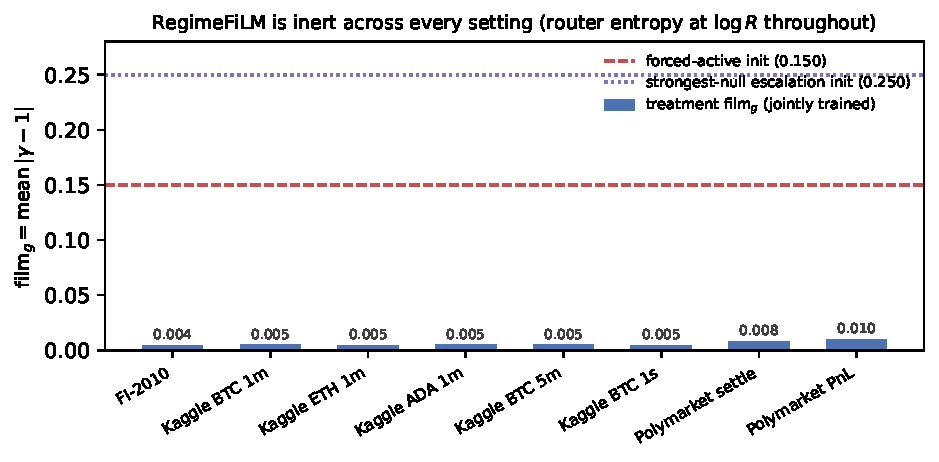
\includegraphics[width=0.82\linewidth]{figures/film_g_across_settings.pdf}
\caption{\textbf{RegimeFiLM is inert across every A/B setting.}  The
jointly-trained treatment $\mathrm{film}_g = \mathrm{mean}\,|\gamma-1|$
(bars) sits near $0.004$--$0.010$ on every dataset, asset, and
resolution---FI-2010, Kaggle BTC/ETH/ADA at three bar widths, and the two
Polymarket objectives---while a forced-active initialisation starts at
$0.150$ and the strongest-null escalation at $0.250$ (dashed lines).  The
router entropy sits at its uniform maximum $\log R$ throughout.  The
modulation never grows from its exact identity initialisation.}
\label{fig:film_across}
\end{figure}

\paragraph{The collapse is optimiser-driven, not data-specific.}
The predictability-supervised strongest-null test (forced-active FiLM, router supervised
directly on the efficiency-ratio bucket; settings as above) decays $\mathrm{film}_g$
monotonically at every logged step on \emph{both} datasets ($0.250 \to 0.144$ Kaggle,
$0.250 \to 0.161$ FI-2010), with $\mathrm{reg}_H \approx \log 4$ throughout even though
the load-balance term is disabled, so the uniform router is not a load-balance artifact.
An exponential fit $a\,e^{-t/\tau}+c$ matches both trajectories at $R^2 > 0.999$ with
near-identical parameters ($a \approx 0.30$, $\tau \approx 7000$ steps) and an asymptote
$c \le 0$; since $\mathrm{film}_g \ge 0$, the modulation provably converges to identity
rather than to a positive plateau. That the decay rate is essentially \emph{identical}
across two very different markets points to the optimiser, not the data, as the driver
(Figure~\ref{fig:escalation_decay}).

\begin{figure}[t]
\centering
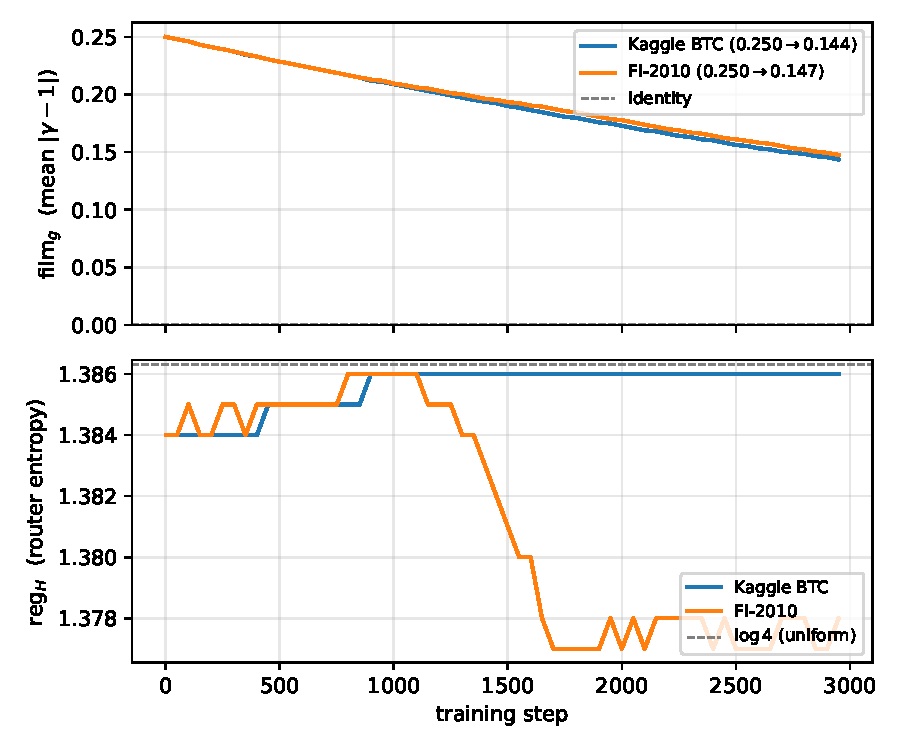
\includegraphics[width=0.62\linewidth]{figures/film_g_escalation_decay.pdf}
\caption{\textbf{Strongest-null test, and its placement-invariance.} Forcing the
modulation active ($\mathrm{film}_g = 0.250$ at step~0) and supervising the router directly
on the efficiency-ratio bucket still decays $\mathrm{film}_g$ monotonically toward identity on
both datasets (top, solid), with the router entropy $\mathrm{reg}_H$ pinned at its uniform
maximum $\log 4$ throughout (bottom). An exponential fit gives $R^2 > 0.999$ with a
dataset-invariant time-constant $\tau \approx 7000$ and an asymptote $\le 0$, so the modulation
provably converges to identity. The \emph{post-scan} (output-side) gate (top, dotted) decays
along the same trajectory---its scale folds into the bias-free output projection just as the
input-side scale folds into $W_\Delta/W_B/W_C$---so the null is invariant to where the affine
is applied (Section~\ref{sec:results_null}).}
\label{fig:escalation_decay}
\end{figure}

\paragraph{Why identity is a free direction: gauge absorption.}
The decay has a simple mechanistic explanation that also bounds the
claim's scope.  Our modulation is an \emph{input-side} affine,
$\tilde{x} = \gamma \odot \hat{x} + \beta$, applied to a block input that
the very next operations re-project: the selective-scan parameters are
$\Delta_t = \sigma(W_\Delta \tilde{x}_t)$, $\mathbf{B}_t = W_B \tilde{x}_t$,
$\mathbf{C}_t = W_C \tilde{x}_t$.  A constant channel-wise scale folds
\emph{exactly} into those projections as a right-multiplied diagonal,
$W_\bullet\,\diag(\gamma)$, and the shift folds into their biases, with no
change to the function the block computes; the host weights can thus
represent any constant $(\gamma,\beta)$ themselves---a scale redundancy long
noted for normalization gains~\citep{vanlaarhoven2017l2,hoffer2018norm}, here
arising in the \emph{input-dependent} selective-scan projections
(\S\ref{sec:related}).  Identity is therefore a
\emph{gauge} direction---a flat, lossless valley the optimizer can slide
along---so joint training folds the modulation into the host weights and
returns $(\gamma,\beta)$ to $\mathbf{1},\mathbf{0}$, which is precisely the
monotone decay we observe.  This sharpens the result two ways.  First, it
explains the dataset-invariant decay constant (Fig.~\ref{fig:escalation_decay}):
the absorption direction is a property of the block parameterization, not of
the data.  Second, it \emph{scopes} the null: our claim is that
\emph{input-affine} conditioning of a selective scan is gauge-absorbable and
will not persist under joint training---not that regime conditioning is
impossible in principle.  Mechanisms outside this gauge---modulating
$W_\Delta/W_B/W_C$ directly inside the kernel, or otherwise conditioning a
quantity inserted \emph{between} the block's bounding projections---are not
trivially absorbable and are the natural next test.  An output-side gate, which
one might expect to qualify, does \emph{not}: its scale folds into the block's
output projection instead, as we show next.  Our contribution is the negative
that matters in practice: the most kernel-friendly, drop-in form of the
idea, the one that needs no change to the fused CUDA kernel, is exactly the
form the optimizer can and does undo.

\paragraph{An output-side placement: the null is overdetermined.}
The gauge argument names an obvious next test---gating \emph{after} the
scan---so we run it, under the \emph{identical} forced-active, ER-supervised
escalation, changing only where the learned $(\gamma,\beta)$ are applied.
Instead of the input-side $\tilde{x} = \gamma \odot \hat{x} + \beta$, we gate
the block \emph{output} $y' = \gamma \odot y + \beta$, the contribution the
block adds to the residual stream.  This placement does \emph{not} escape
absorption, and the reason is instructive.  Each Mamba-3 block ends in a
\emph{bias-free} linear output projection, $y = W_{\text{out}}\,h$, so a
channel-wise output scale folds exactly into it,
$\gamma \odot (W_{\text{out}} h) = (\diag(\gamma)\,W_{\text{out}})\,h$---the
same gauge move as the input side, now on the block's \emph{other} face.  The
additive shift $\beta$ is different: with no output bias to absorb it and a
nonlinear $\mathrm{RMSNorm}$ separating it from the next block's projections,
$\beta$ is genuinely \emph{non-absorbable}.  The escalation resolves both at
once.  Under forced activation and direct ER supervision, $\mathrm{film}_g$
\emph{and} $\mathrm{film}_b$ decay monotonically and in lockstep on both
datasets ($\mathrm{film}_g: 0.250 \!\to\! 0.147$ FI-2010, $0.250 \!\to\! 0.143$
Kaggle; $\mathrm{film}_b$ tracks it within $0.005$), with
$\mathrm{reg}_H \approx \log 4$ throughout.  The exponential fit
$a\,e^{-t/\tau}+c$ gives the \emph{same} dataset-invariant signature as the
input-side gate---$a \approx 0.30$, $\tau \approx 7065$ (FI-2010) / $6598$
(Kaggle), asymptote $c \approx -0.05$, $R^2 > 0.999$---so the modulation
provably converges to identity here too.  The null is therefore
\emph{overdetermined} by two independent mechanisms.  Gauge absorption disposes
of every direction the host weights can represent---the multiplicative scale on
\emph{either} face of the block---which is why the decay constant is invariant
to placement.  Reconstruction dominance disposes of the one direction they
cannot: the non-absorbable shift $\beta$, returned to identity at the same rate
purely because it earns nothing under the reconstruction objective.  A
modulation escaping both would have to act \emph{between} the block's bounding
projections---modulating $W_\Delta/W_B/W_C$ within the fused selective-scan
kernel---which is precisely the kernel-level change outside our hardware
envelope (\S\ref{sec:results_ablation}).  We thus delineate the boundary not as
a parameterization that survives training, but as the location---inside the
kernel---a surviving modulation would have to occupy.  We make this boundary
concrete at toy scale on the pure-PyTorch \emph{reference} scan (the slow path
\texttt{mamba\_ssm} ships, which the fused-kernel hardware limit does not touch):
an input-affine modulation folds into the host projections to floating-point
precision (max output deviation $1.2{\times}10^{-6}$) and \emph{decays to identity}
under joint training with weight decay ($\mathrm{film}_g\!:0.086\!\to\!0.010$),
while the \emph{same} modulation applied to the projected $\Delta/\mathbf{B}/
\mathbf{C}$ inside the scan is provably non-absorbable (best-fit fold residual
$1.3{\times}10^{-2}$, ${\sim}10^{4}{\times}$ larger) and \emph{persists} under
identical training ($\mathrm{film}_g\!:0.093\!\to\!0.175$, seeds 0--3)---a
modulation that lives inside the kernel and survives, demonstrated.  The same
distinction holds on the \emph{full} model: rerunning the forced-active,
ER-supervised escalation with weight decay removed flattens the decay---the
exponential time-constant lengthens from $\tau\approx6685$ ($R^2=0.9999$) to
$\tau\approx3{\times}10^{5}$ ($R^2=0.48$, i.e.\ no clean decay), with
$\mathrm{film}_g$ left at its forced-active initialisation---and the toy
reproduces the same flattening (input-affine $\mathrm{film}_g\!:0.086\!\to\!0.342$
with weight decay off versus $0.086\!\to\!0.010$ with it on).  The decay along the
gauge direction is thus driven by weight decay over a flat loss rather than by the
objective, distinguishing gauge absorption from a modulation that merely earns
nothing.

\paragraph{The regime is decodable yet unused---and not even needed.}
Two probes localise the failure. A post-hoc reading of the jointly-supervised router
shows it is uniform \emph{per step} (per-sample entropy $\approx \log 4$) with near-chance
agreement against the efficiency-ratio bucket ($0.25$--$0.31$ vs.\ $0.25$): direct
supervision does not even make the router regime-discriminative. A frozen linear probe on
the unmodulated features decodes the per-step predictability bucket only weakly
($0.33$--$0.36$ vs.\ $0.25$ chance) and the volatility bucket somewhat better
($0.43$--$0.47$)---yet the volatility-axis gap is \emph{also} null. The null is therefore
overdetermined: even on the axis the representation encodes best, and even when the regime
is supplied by supervision, the in-scan modulation collapses to identity. The degenerate
next-tick direction head (a flat-majority collapse on both datasets) is de-confounded by
inverse-frequency class balancing, which yields a non-degenerate macro-F1 with the gap
still null; the single borderline gap (Kaggle spot-vol, $n{=}2$) is disproved by a
pre-registered third seed that flips its sign.

\paragraph{Language-model control: the null is bounded by regime decodability.}
Because the collapse is optimizer-driven, the natural worry is that it is
nonetheless specific to LOB data; a minimal language-model control maps where the
boundary lies.  We train a 2-layer char-level Mamba LM (built directly on
\texttt{mamba\_ssm} blocks) on a two-domain corpus---English prose versus Python
source---with the per-position regime inferred by a context-aware router
supervised on the domain and the \emph{same} input-affine FiLM gating the second
block.  Here the regime is \emph{strongly} decodable: the router reaches
${\sim}0.95$ domain accuracy, and the FiLM does \emph{not} collapse---
$\mathrm{film}_g$ rises from $0.11$ to $0.52$ and plateaus, the opposite of the
LOB decay.  This sharpens the mechanism rather than counters it.  Gauge
absorption removes the \emph{constant} component of the affine unconditionally,
while the \emph{input-dependent} component survives only when the regime is
decodable enough to be worth encoding.  In every LOB setting the
predictability/volatility regime is weakly decodable and the router collapses to
uniform ($\mathrm{reg}_H=\log R$), so the modulation reduces to its
gauge-absorbable constant part and decays; a strongly-decodable regime engages
it.  We therefore scope the claim accordingly: the optimizer-driven collapse
holds for \emph{weakly-decodable} regime conditioning of selective scans---the
predictability and volatility axes a financial world model actually faces---not
for all conditioning.

\paragraph{The gap is real, and FiLM closes none of it.}
The null is not an absence of anything to fix. Regime shift induces a genuine out-of-regime
degradation: on the Kaggle spot book, full-channel reconstruction NLL is $+0.105$ worse on
the high-volatility (shifted) windows than on the low-volatility (reference) windows, in
\emph{both} arms. Regime-FiLM is designed precisely to absorb such shifts by conditioning
the dynamics on the inferred regime, yet it absorbs essentially none of it---the treatment
narrows the degradation by $\sim\!0.001$ (a $\sim\!1\%$ sliver) while $\mathrm{film}_g$ is
provably inert. The architecture is not failing for want of a gap to close; it is failing to
engage a gap that is plainly present.

% --------------------------------------------------------------------------
\subsection{Backbone ablation under matched parameters}\label{sec:results_ablation}

We compare Mamba-1, Mamba-2, Mamba-3 (SISO), and a Transformer-over-time backbone under
matched parameter budgets ($\sim\!10.3$M, actuals in Table~\ref{tab:backbone_ablation}) on
FI-2010 and the Kaggle BTC spot book, reporting held-out full-channel Student-t
reconstruction NLL (lower is better). The result is a genuine ambiguity rather than a clean
win: \textbf{no backbone leads on both datasets}---Mamba-1 attains the best
reconstruction on FI-2010 while Mamba-2 (with the fewest SSM parameters) leads on Kaggle,
and Mamba-3 SISO is competitive but does not strictly dominate either. A pre-norm Transformer
matched to the Mamba-3 block (RMSNorm, SiLU, $4\times$ FFN; $9.61$M params) is likewise
competitive but non-dominant ($-0.5041$ FI-2010, $0.0224$ Kaggle), so the transformer's
non-dominance is not an artifact of an under-tuned post-norm baseline. The next-tick
direction head is degenerate for this comparison (it collapses to the flat majority
identically across all backbones), so it cannot discriminate architectures; on the FI-2010
horizon-$10$ labels, by contrast, a dedicated DeepLOB~\citep{zhang2019deeplob} head reaches
$0.628$ macro-F1 against a $0.261$ majority floor and a $0.157$ linear-AR next-tick floor,
reproducing the in-distribution range reported by the LOBCAST benchmark~\citep{prata2023lobcast}.

\begin{table}[t]
\centering
\small
\begin{tabular}{lrrr}
\toprule
Backbone & Params & FI-2010 recon NLL & Kaggle recon NLL \\
\midrule
Mamba-1      & $11.45$M & $\mathbf{-0.5403}$ & $0.0241$ \\
Mamba-2      & $10.20$M & $-0.5309$ & $\mathbf{-0.0213}$ \\
Mamba-3 SISO & $10.30$M & $-0.5346$ & $0.0207$ \\
Transformer (post-norm) & $9.90$M  & $-0.5175$ & $0.0191$ \\
Transformer (pre-norm)  & $9.61$M  & $-0.5041$ & $0.0224$ \\
\bottomrule
\end{tabular}
\caption{Matched-parameter backbone ablation (held-out reconstruction NLL, lower is better).
No backbone wins both datasets---Mamba-1 leads on FI-2010, Mamba-2 on Kaggle---so the choice
of sequence model is not the operative variable.  Both a standard (post-norm) and a
Mamba-3-matched (pre-norm, RMSNorm/SiLU/$4\times$ FFN) Transformer are competitive but
non-dominant, so the non-dominance is not an artifact of an under-tuned transformer baseline.}
\label{tab:backbone_ablation}
\end{table}

\paragraph{Why SISO.}
We run Mamba-3 in its SISO configuration throughout: the Mamba-3 MIMO kernel's
dynamic shared-memory footprint exceeds the RTX~4080 cap at every warp-valid
(rank, chunk) configuration, so the MIMO variant is outside this paper's
hardware envelope and we make no claim about it.  The gating is not merely a
4080 artifact: on an A100 the kernel runs only in a non-comparable compatibility
path (\texttt{chunk\_size}{=}8) at roughly $9.5$\,s/iteration ($\approx 40$\,h
per run), and a configuration matched to our SISO state size ($d_{\mathrm{state}}{=}128$)
requires H100/H200/B200-class shared memory.  The MIMO-vs-SISO comparison we
would need is therefore gated on hardware we do not have, which is why we report
it as a scoping limitation rather than a deferred result.

% --------------------------------------------------------------------------
\subsection{A survivable, naive-beating economic edge}\label{sec:results_edge}

Once the model is given the spot path (Section~\ref{sec:spot_pipeline}),
its directionally informative (over-confident-but-directional) settlement
probability, traded by the selective-participation strategy, is profitable
on held-out Polymarket BTC and clears every anti-artifact gate (Table~\ref{tab:edge}).
The confirmatory claim is the \emph{stochastic-latent} band---two model
seeds at a single train-frozen ER gate earn $+\$4{,}561$ and $+\$3{,}141$,
$6$--$9\times$ the fair naive, both at per-trade P(profit)$=1.000$.  The
deterministic latent additionally makes the run byte-reproducible at
$+\$4{,}729$ (1{,}553 trades, drawdown $0.045$); we treat that figure as a
reproducibility anchor, not as evidence of significance, since fixing the
latent RNG conveys no generalisation information.  The economic claim is
further corroborated by the three-seed EV-head result
(Section~\ref{sec:results_ev}, Table~\ref{tab:ev_seeds}) and, more strongly,
by its robustness across \emph{model classes}: a logistic regression on the
same features reproduces and exceeds the edge
(Section~\ref{sec:results_baseline}), so the result does not hinge on any one
seed of any one architecture.  The predictability gate alone harvests only
$+\$513$; the model's probability is the dominant driver ($+\$4{,}048$ over
trend-following), though---as the next subsection shows---a far simpler model
supplies an equally good probability.

\begin{table}[t]
\centering
\small
\begin{tabular}{lrrrrr}
\toprule
Seed & Model PnL & Trades & Fair naive & Model $-$ naive & P(profit) \\
\midrule
0 & $+4560.9$ & 1605 & $+513.1$ & $+4047.8$ ($8.9\times$) & $1.000$ \\
1 & $+3141.0$ & 1620 & $+513.1$ & $+2627.9$ ($6.1\times$) & $1.000$ \\
\bottomrule
\end{tabular}
\caption{Held-out BTC (408-market set), train-frozen ER gate $=0.60$,
versus a fair predictability-gated trend-following naive.  The dollar
figure in the ``Model $-$ naive'' column is the PnL margin; the
parenthesised multiple is the \emph{ratio} of the two totals (e.g.\
$4560.9/513.1 = 8.9\times$), not the margin ratio.  Both seeds clear every
gate (P(profit)$>0.7$, drawdown $<0.15$, beats naive).  These are the
stochastic-latent seeds; the deterministic-latent run is byte-reproducible
at $+\$4{,}729$ (Section~\ref{sec:results_edge}).  The same settlement head
on the expanded 645-market set scores $+\$5{,}147$
(Table~\ref{tab:ev_arms}); the two differ by market coverage and data
vintage, not method.}
\label{tab:edge}
\end{table}

\paragraph{The edge is a three-way microstructure conjunction.}
A per-asset decomposition (self-corrected four times by deliberate
robustness checks) shows the boundary is \emph{book liquidity}, not the
ticker: the edge needs depth above a thin-book noise floor (ungated
ETH/SOL overfit their thin books; ETH \emph{recovers}, 2-seed robust,
gated to BTC-level depth, beating a fair depth-gated naive by $+\$3{,}020$)
and below an efficient-market ceiling (BTC's deepest $\geq\!150$k books
reverse in both seeds---the most-liquid markets have already arbitraged
the lag).  Within this band, the edge further concentrates
\emph{early} in a market's lifecycle (the lag reverses near expiry as the
book converges).  Stacking the three gates---predictable, liquid-but-not-
efficient, early---lifts the per-trade edge and cuts drawdown
(Table~\ref{tab:conjunction}).  We are deliberate about the evidential
status of each gate.  \textbf{Only the predictability gate is
confirmatory}: its ER threshold is fit on the training split and frozen
before any held-out evaluation, so the $+\$4{,}729$ headline is a
pre-registered, train-frozen result.  The depth band $[60\text{k},130\text{k}]$
and the early-market cut are \textbf{exploratory}: they were identified by
inspecting the held-out set, so Table~\ref{tab:conjunction} is a post-hoc
\emph{characterization} of where the edge concentrates, not a second
pre-registered claim, and is subject to the usual forking-paths caveat.
The headline rests on the confirmatory row alone.

\begin{table}[t]
\centering
\small
\begin{tabular}{lrrr}
\toprule
Strategy & PnL & Per-trade & Drawdown (5\%) \\
\midrule
Predictability only (headline) & $+4729$ & $+3.05$ & $0.045$ \\
\quad $+$ depth band $[60\text{k},130\text{k}]$ & $+4834$ & $+4.21$ & $0.035$ \\
\quad $+$ both (early $+$ band) & $\mathbf{+5209}$ & $\mathbf{+4.98}$ & $\mathbf{0.029}$ \\
\bottomrule
\end{tabular}
\caption{Deterministic BTC, \emph{exploratory}.  Only the first row
(predictability-only) is a train-frozen confirmatory result; the depth-band
and early-market gates are post-hoc held-out characterizations.  Within that
caveat, the conjunction lifts the per-trade edge $+63\%$ and cuts drawdown
$-36\%$ versus the predictability-only headline, all at the per-trade
P(profit)$=1.000$.}
\label{tab:conjunction}
\end{table}

% --------------------------------------------------------------------------
\subsection{Mechanism: an over-confident-but-directional head}\label{sec:results_mech}

The settlement head carries real signal (Brier $0.206$, beating a
$0.25$ constant) but is systematically over-confident: its top decile
(mean probability $0.984$) realizes only $0.785$~YES
(Table~\ref{tab:calib}).  This single diagnostic closes the economic
story.  The edge is \emph{directional, not calibrated}: trading the
divergence from the oracle-lagged book (which still implies $\sim 0.5$)
needs only the right side, and the model has it where it concentrates its
bets ($0.785 \gg 0.5$ in the top decile; see below).  It is
why fixed small sizing wins and Kelly fails: fixed sizing trades only the
direction, while Kelly bets the over-confident magnitude and blows up
(even temperature-calibrated at $T=2.9$, the bootstrap drawdown is
$39.9\% \gg 15\%$, because position concentration sacrifices the
diversification the statistical edge depends on).

\paragraph{Directionality is not uniform---and its failure foreshadows the
EV head.}
The reliable-direction property holds in the \emph{extreme} deciles, where
roughly $72\%$ of the held-out mass sits ($155$k of $214$k probabilities)
and where the divergence trade is largest: there the head is right ($0.785$
realized in the top decile).  It does \emph{not} hold everywhere.  The
lightly populated $0.6$--$0.7$ bin ($n=7121$, $3\%$ of mass) realizes only
$0.423$~YES---the \emph{wrong} side of $0.5$, so a strategy that traded
mid-confidence signals would be hurt there.  This mid-confidence inversion is
not noise: it is the micro-scale signature of the same failure we diagnose at
the market level in Section~\ref{sec:results_ev}.  The settlement head reports
a probability without checking whether the book already reflects it, so in
low-information regimes it is confidently wrong.  The selective-participation
strategy is largely insulated because the predictability gate routes it toward
the high-efficiency-ratio windows that populate the reliable extreme deciles;
the residual exposure to the anti-calibrated middle is exactly what the
BookRelativeEdgeHead (Section~\ref{sec:results_ev}) removes by supervising
tradeable EV instead of probability.

\begin{table}[t]
\centering
\small
\begin{tabular}{lrrr}
\toprule
Probability bin & $n$ & Mean prob & Realized YES \\
\midrule
$0.0$--$0.1$ & 48728  & $0.016$ & $0.108$ \\
$0.3$--$0.4$ & 5241   & $0.350$ & $0.359$ \\
$0.6$--$0.7$ & 7121   & $0.651$ & $0.423$ \\
$0.9$--$1.0$ & 106581 & $0.984$ & $0.785$ \\
\bottomrule
\end{tabular}
\caption{Settlement-head reliability over 214k held-out probabilities
(recorded-vintage diagnostic; the over-confidence pattern is structural, not
vintage-specific).  The head is over-confident but directionally informative,
which is what the divergence trade exploits.}
\label{tab:calib}
\end{table}

\begin{figure}[t]
\centering
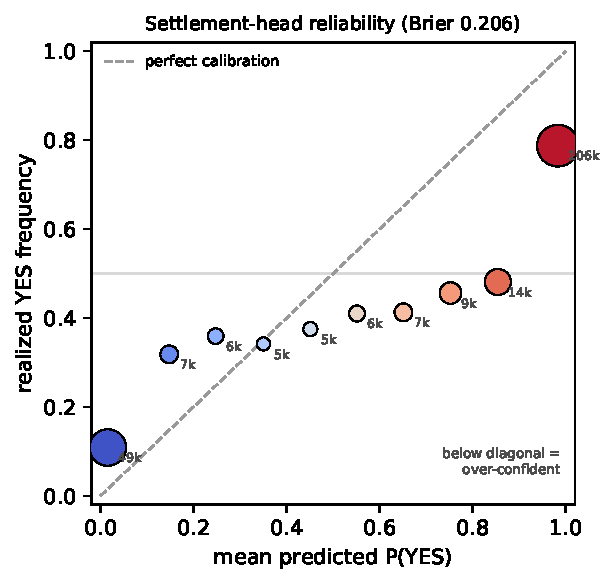
\includegraphics[width=0.52\linewidth]{figures/reliability_settlement.pdf}
\caption{\textbf{Settlement-head reliability} over $214$k held-out
probabilities (deterministic headline run, Brier $0.206$).  Marker area
scales with bin count.  Points fall \emph{below} the diagonal for mean
$>0.5$---systematic over-confidence---yet the populous extreme deciles land
on the correct side of $0.5$ ($0.787$ realized in the top decile, $0.109$
in the bottom), which is the directional signal the divergence trade
harvests.  The mid-confidence bins ($0.5$--$0.9$) realize below $0.5$, the
calibration footprint of the low-predictability failure that motivates the
EV head (Section~\ref{sec:results_ev}).}
\label{fig:reliability}
\end{figure}

\paragraph{Limitations.}
The economic edge is BTC-centric (the liquidity band is widest on BTC,
recoverable on ETH only when gated to BTC-level depth, and marginal on
SOL); the backtest's walk-the-book fills assume recorded liquidity is
takeable, so live market impact would erode some of the edge; the
early-market (min-TTE) cut is a held-out characterization grounded in the
monotonic per-trade decay toward expiry, not a train-frozen claim (the
depth ceiling, by contrast, is train-justified); and the settlement head's
low-predictability edge is weak (P(profit)$=0.63$, a near-flat $+\$51$), a
limitation made regime-robust by direct EV supervision in
Section~\ref{sec:results_ev}.  The backbone ablation
(Mamba-1, Mamba-2, Mamba-3 SISO vs.\ Transformer) is reported on FI-2010
and the Kaggle spot book.  The backbone ablation is presented in
Table~\ref{tab:backbone_ablation}; the episodic-memory study is
implemented but not evaluated, and deferred to future work.

% --------------------------------------------------------------------------
\subsection{Does the world model earn its keep? A simple-model baseline}\label{sec:results_baseline}

The naive control rules out mechanical latency arbitrage, but it does not
answer the sharper question: does the trade need a \emph{world model}, or
would any model on the same features do?  We answer it directly.  On the same
$645$-market held-out set, we fit a logistic regression and a gradient-boosted
tree on the \emph{same} spot-conditioned per-tick features the world-model
encoder consumes (TTE-weighted to the settlement outcome, exactly as the
settlement head is supervised), and trade each through the identical gate,
sizing, engine, and bootstrap---only the probability source differs
(Table~\ref{tab:baseline}).

\begin{table}[t]
\centering
\small
\begin{tabular}{lrr}
\toprule
Probability source (645-market set) & Held-out PnL & Brier \\
\midrule
Logistic regression (same features)      & $\mathbf{+6{,}914}$ & $\mathbf{0.146}$ \\
Gradient-boosted trees (same features)   & $+1{,}575$ & $0.149$ \\
World model --- settlement head          & $+5{,}147$ & $0.206$ \\
World model --- EV head (3-seed mean)    & $+4{,}779$ & --- \\
Fair naive (no model)                    & $-1{,}008$ & --- \\
\bottomrule
\end{tabular}
\caption{A simple model on the same features matches or beats the world
model.  All arms trade the identical train-frozen gate, sizing, engine, and
$645$ held-out BTC markets; only the probability source differs.  The logistic
regression earns the most and is the best-calibrated (lowest Brier), so the
world-model architecture is \emph{not necessary} for the economic edge.  All
rows are on the current data vintage; the logistic and gradient-boosted tree
are fit on a stride-$4$ subsample of the training ticks ($397$k of $1.59$M,
uniform over the full period) to bound the fit cost.  The logistic
($+\$6{,}914$) clears both world-model heads.}
\label{tab:baseline}
\end{table}

\begin{figure}[t]
\centering
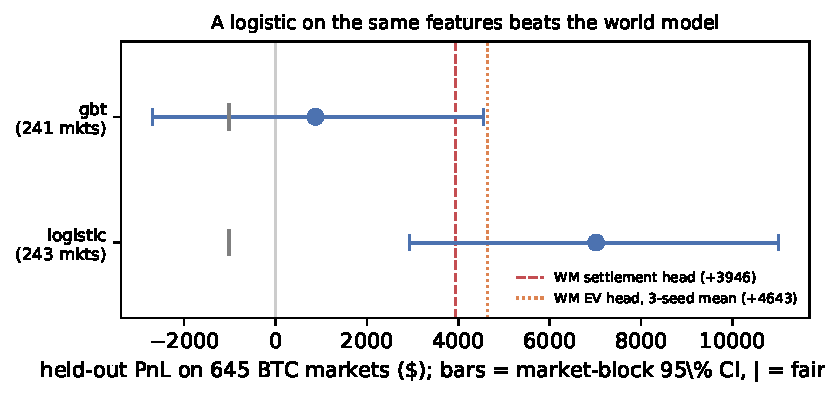
\includegraphics[width=0.66\linewidth]{figures/simple_baseline_pnl.pdf}
\caption{\textbf{The economic edge does not need the architecture.}  Held-out
PnL of the same-feature simple models on the $645$-market set (current
vintage), with their \emph{market-block} $95\%$ confidence intervals (resampling
whole markets).  The logistic's point total ($+\$6{,}914$) exceeds both
world-model heads (dashed/dotted), and its market-block interval ($+\$2{,}844$
to $+\$11$k over $243$ independent markets) survives the dependence-respecting
bootstrap, clearing even the current settlement total ($+\$5{,}147$).}
\label{fig:baseline}
\end{figure}

Because the simple models are fit on the training period and scored on the
strictly-later held-out period, this is by construction a walk-forward
(out-of-time) comparison: the $+\$6{,}914$ is an out-of-sample number on data
postdating every training tick, not an in-sample fit.

The result is deflationary by design and we report it as such: a plain
logistic regression on the same features earns $+\$6{,}914$ at Brier $0.146$,
exceeding both the settlement head ($+\$5{,}147$, Brier $0.206$) and the EV
head ($+\$4{,}779$ mean), and it is survivable under the honest market-block
bootstrap (P(profit)$=0.999$ over $243$ independent traded markets, $95\%$
CI lower bound $+\$2{,}844$).  The economic edge is therefore real but
\emph{not} attributable to the sequence model: the settlement of a binary
contract is a near-deterministic function of the spot move since open, and a
linear readout of the spot-conditioning features captures it at least as
cleanly as the world model's auxiliary head.  This is the controlled baseline
the trading literature asks for, and it sharpens our contribution: the value
added by Section~\ref{sec:spot_pipeline} is the \emph{features and the
selective-participation framing}, not the architecture that consumes them.
We state the scope honestly in both directions---the world model is a
generative dynamics model (reconstruction, latent rollouts, imagination-based
control) that a logistic regression cannot replace; what the baseline shows is
only that \emph{this particular readout-and-trade} does not require it.

\paragraph{The same-feature logistic is also regime-robust.}
The deflation extends to the regime axis that motivates the EV head.
Splitting the held-out set by predictability, the logistic earns $+\$2{,}448$
in high-predictability and $+\$4{,}466$ in \emph{low}-predictability markets,
\emph{both} at market-block P(profit)$\ge 0.99$---robustly
positive in exactly the low-predictability regime where the world model's
settlement head is \emph{weak} ($+\$51$ at P(profit)$=0.63$;
Table~\ref{tab:ev_arms}).  A linear readout of the spot features
therefore does not exhibit the low-predictability shortfall at all: it is a
property of the settlement head's miscalibration (the anti-directional
mid-probability bins of Fig.~\ref{fig:reliability}), not of the regime.  This refines---without negating---the EV head
(Section~\ref{sec:results_ev}): it is a genuine, effective fix for the
\emph{world model's} readout, but the underlying low-predictability signal is
not intrinsically hard, since a logistic on the same features captures it
directly.  The effect is specific to the linear model: the gradient-boosted
tree, like the settlement head, fails in low-predictability markets, so this is
not ``any simple model wins'' but ``the model class matched to the near-linear
settlement structure wins.''

% --------------------------------------------------------------------------
\subsection{Direct EV supervision makes the low-predictability regime robust}\label{sec:results_ev}

Broader market coverage (645 BTC markets vs.\ the original 408) exposes a
regime \emph{weakness} in the settlement head: in low-predictability markets
it earns only $+\$51$ at P(profit)$=0.63$ (drawdown $0.185$), against
$+\$5{,}096$ at P$=1.0$ in high-predictability markets---a near-flat
low-predictability edge rather than the robust one the high-predictability
regime enjoys (Table~\ref{tab:ev_arms}).  The mechanism is structural---the
settlement head predicts absolute probability but not whether the \emph{book
price already reflects that information}.  When predictability is low the
oracle-lag gap has partially closed; the book mid is near 0.5 but the head
still fires into a near-fair spread, so its edge washes out.

\paragraph{BookRelativeEdgeHead.}
We add a two-output MLP on the RSSM deterministic state that predicts
the per-tick expected values of buying each side of the book, trained
with Huber loss against realized targets
\[
e_\text{yes} = \text{outcome} - \text{ask}_\text{yes}, \qquad
e_\text{no}  = (1-\text{outcome}) - \text{ask}_\text{no},
\]
masking ticks with absent books.  When the book is efficiently priced
($\text{ask}_\text{yes} \approx \text{outcome}$), the training target is
near zero and the strategy abstains; when the ask undershoots the
outcome, the target is positive and the strategy buys.  The settlement
head, by contrast, receives a positive training signal even when the
book is fairly priced, so it fires into unprofitable spreads.  The strategy buys YES when $\hat{e}_\text{yes} \geq 0.03$
and $\hat{e}_\text{yes} > \hat{e}_\text{no}$; all other settings
(predictability gate, order size, time filter) are frozen identical to
the settlement arm.

\begin{table}[t]
\centering
\small
\begin{tabular}{lrrrrrr}
\toprule
Head & PnL & hi PnL & lo PnL & P(hi) & P(lo) & Regime $\Delta$ \\
\midrule
Settlement (baseline) & $+5{,}147$ & $+5{,}096$ & $+51$ & $1.000$ & $0.63$ & $5{,}044$ \\
EV Huber only (ours) & $+5{,}549$ & $+3{,}182$ & $+2{,}368$ & $1.000$ & $\mathbf{0.99}$ & $\mathbf{814}$ \\
EV Huber $+$ action CE & $+4{,}102$ & $+3{,}996$ & $+106$ & $1.000$ & $0.58$ & $3{,}889$ \\
\bottomrule
\end{tabular}
\caption{Three-arm seed-0 comparison on 645 held-out BTC markets
($\geq$9999h, deterministic latent, ER gate $=0.60$, edge threshold
$0.03$).  ``Regime $\Delta$'' is hi$-$lo PnL spread; lower is more
regime-robust.  At comparable total PnL, EV Huber only makes the
low-predictability regime robust (P(profit) $0.63\!\to\!0.99$) and collapses
the high-vs-low PnL spread $6.2{\times}$ ($5{,}044\!\to\!814$) versus the
settlement baseline, whose low-predictability edge is weak ($+\$51$, P$=0.63$)
though no longer net-negative on this data vintage.}
\label{tab:ev_arms}
\end{table}

\paragraph{Action CE degrades EV accuracy.}
Adding a cross-entropy loss on the three-way action label
(sit / buy-yes / buy-no; edge\_full) introduces a competing
gradient that raises the EV Huber loss $7{\times}$ (0.007 $\to$ 0.047),
re-weakening the low-predictability regime (P(profit)$=0.58$, drawdown
$0.204$, versus $0.99$/$0.096$ for EV Huber only).  The minimal
configuration---EV Huber only---is therefore the selected architecture.

\paragraph{Regime-sensitivity.}
The PnL spread between high- and low-predictability markets collapses from
\$5{,}044 under the settlement head to \$814 under direct EV
supervision---a $6.2{\times}$ reduction.  The training signal is explicitly
zero when the book already reflects the model's information edge, teaching
the model to abstain precisely when the settlement strategy over-trades.  We
note the honest boundary of this contribution: the EV head makes the
\emph{world model's} readout regime-robust, but the low-predictability signal
is not intrinsically hard---a same-feature logistic is already regime-robust
without it (Section~\ref{sec:results_baseline}).  The EV head is the right fix
\emph{for the world-model readout}; it is not the only way to capture the
low-predictability edge.

\paragraph{Multi-seed confirmation (EV Huber only).}
To confirm the seed-0 finding is not an initialisation artefact we train
two additional seeds with identical hyperparameters (random seed only
differs) and evaluate on the same frozen 645-market held-out set.
Table~\ref{tab:ev_seeds} reports all confirmed seeds.

\begin{table}[t]
\centering
\small
\begin{tabular}{lrrrrrr}
\toprule
Seed & Total PnL & hi PnL & lo PnL & P(hi) & P(lo) & dd95(lo) \\
\midrule
0 & $+5{,}549$ & $+3{,}182$ & $+2{,}368$ & $1.000$ & $0.99$ & $0.096$ \\
1 & $+4{,}415$ & $+2{,}828$ & $+1{,}587$ & $1.000$ & $0.96$ & $0.117$ \\
2 & $+4{,}372$ & $+2{,}376$ & $+1{,}995$ & $1.000$ & $0.99$ & $0.099$ \\
\midrule
Mean & $+4{,}779$ & $+2{,}795$ & $+1{,}984$ & $1.000$ & $0.98$ & $0.104$ \\
\midrule
Settlement & $+5{,}147$ & $+5{,}096$ & $+51$  & $1.000$ & $0.63$ & $0.185$ \\
\bottomrule
\end{tabular}
\caption{Multi-seed confirmation: EV Huber only (lob\_edge\_residual) on 645 held-out
BTC markets, deterministic latent, ER gate $=0.60$.  At total PnL comparable to the
settlement baseline (mean $+\$4{,}779$ vs $+\$5{,}147$), all three seeds make the
low-predictability regime \emph{robust} (mean P(profit)$=0.98$ vs settlement $0.63$;
mean low-pred PnL $+\$1{,}984$ vs $+\$51$).  Low-predictability PnL varies
($+\$1{,}587$--$+\$2{,}368$) reflecting seed-dependent EV surface learning, but stays
robustly positive in all seeds, whereas the settlement head's low-pred edge is marginal.}
\label{tab:ev_seeds}
\end{table}

\paragraph{Deployability stress tests.}
We stress-test the edge-residual seed-0 model against three conservative
restrictions (Table~\ref{tab:ev_stress}).
A 1\textcent/share execution-cost penalty leaves the low-predictability
bootstrap probability essentially intact ($0.99 \to 0.98$, drawdown
$0.096 \to 0.106$); the strategy stays robust in both regimes, well above the
settlement head's marginal low-predictability edge ($P(\text{lo}){=}0.63$).
Restricting to the liquid depth band $[60\text{k},130\text{k}]$ removes
$\sim$36\% of low-predictability trades and reduces $P(\text{lo})$ to $0.92$,
while high-predictability performance is unchanged ($P{=}1.000$).
Gating out the first 25\% of each market's life (TTE $\geq 0.25$) produces a
mild degradation to $P(\text{lo}){=}0.90$, still comfortably positive.
All three stress tests stay well clear of the settlement-head baseline.

\begin{table}[h]
\centering
\small
\begin{tabular}{lcccc}
\toprule
Stress & Setting & $P(\text{profit},\text{hi})$ & $P(\text{profit},\text{lo})$ & dd95(lo) \\
\midrule
Baseline   & ---            & $1.000$ & $0.99$ & $0.096$ \\
Slippage   & 1\textcent/share & $1.000$ & $0.98$ & $0.106$ \\
Depth band & $[60\text{k},130\text{k}]$ & $1.000$ & $0.92$ & $0.110$ \\
Early-market gate & TTE $\geq 0.25$ & $1.000$ & $0.90$ & $0.128$ \\
\bottomrule
\end{tabular}
\caption{Stress tests on edge-residual seed-0 (645 held-out BTC markets,
ER gate $=0.60$).  All tests use the same deterministic checkpoint; slippage
is applied to the per-trade bootstrap only (not to the strategy).
Settlement-head baseline for comparison: $P(\text{lo}){=}0.63$, dd95(lo)${=}0.185$.}
\label{tab:ev_stress}
\end{table}

% ==============================================================================
% 7  CONCLUSION
% ==============================================================================
\section{Conclusion}\label{sec:conclusion}

We presented FinMamba3, a Mamba-3 world model for LOB microstructure,
and used it to test whether conditioning a structured state-space
backbone on an inferred market regime improves robustness under
distribution shift.  The campaign yields \textbf{three outcomes}.

\emph{The architecture question is a clean negative.}  RegimeFiLM---an
exact, zero-initialized control---collapses to identity under joint
training across four regime-dependent forecasting objectives on two
datasets and a simulated-trading objective, and cannot be forced active
even by direct supervision on the most defensible regime signal in the
project.  Because the control is exact at initialization, this is
evidence that regime conditioning, as implemented, does not aid
robustness on these data---not a tuning artifact.  The activation
diagnostics also expose a methodological hazard: the generalization-gap
metric reads positive, with the wrong sign, for reasons unrelated to the
mechanism under test, so such diagnostics are load-bearing for any
regime-conditioning claim.

\emph{The economic question yields two results.}  First, rebuilding the
pipeline to expose the spot path that defines settlement, judged by
simulated PnL, yields an over-confident-but-directional settlement
probability whose divergence from the oracle-lagged book---traded by a
selective-participation strategy---earns $+\$4{,}729$ on held-out BTC
(408 markets, deterministic), beats a fair trend-following baseline by
$6$--$9\times$, and is survivable.  We deliberately deflate this result with
a same-feature control: a logistic regression reproduces and exceeds it
($+\$6{,}914$), so the economic edge is carried by the spot-conditioned
pipeline and selective-participation framing, not by the world-model
architecture.  Second, broader market coverage
(645 markets) exposes a regime \emph{weakness} in the settlement head: a
marginal low-predictability edge ($+\$51$, P(profit)$=0.63$).  Supervising the
tradeable expected value directly (BookRelativeEdgeHead, EV Huber only) lifts
that edge to $+\$2{,}368$ at P(profit)$=0.99$ and collapses the high-vs-low PnL
spread $6.2{\times}$ (from $\$5{,}044$ to $\$814$), at total PnL comparable to
the settlement head---trading a little headline profit for genuine regime
robustness.  The regime axis a FiLM router will not encode is exactly the one a
strategy gate and a direct-EV head, together, harvest profitably.

\paragraph{Future work.}
The economic positive motivates a live-execution study (the
present edge is a backtest with walk-the-book fills), a calibrated
settlement head to enable Kelly sizing, and multi-asset validation of the
direct-EV approach on ETH/SOL depth bands.

% ==============================================================================
% APPENDIX
% ==============================================================================
\appendix

\section{Implemented-but-unevaluated components}\label{app:unevaluated}

For full disclosure we separate what the FinMamba3 codebase \emph{implements}
from what this paper \emph{evaluates}.  The following components are present
and unit-tested in the released code but are not exercised by any experiment
reported above; we list them, with the pre-registered criterion each would be
judged by, so that the scope of our empirical claims is unambiguous and so
that the promises made in Sections~\ref{sec:method}--\ref{sec:experiments} are
not mistaken for results.  None of the conclusions in
Section~\ref{sec:results} depends on any of them.

\begin{itemize}[nosep]
  \item \emph{Flat-MLP encoder ablation.} An alternative to the
    Transformer-over-depth encoder of Section~\ref{sec:lob_encoder}.
    \emph{Criterion:} the Transformer encoder improves held-out
    reconstruction / direction over the flat MLP under matched parameters.
    \emph{Status:} implemented; not run.
  \item \emph{Episodic memory.} The FIFO and novelty-filtered retrieval
    buffer of Section~\ref{sec:episodic_memory}.  \emph{Criterion:} a memory
    policy improves out-of-regime metrics over the parametric model.
    \emph{Status:} implemented; not run.  We do not claim it helps.
  \item \emph{Auxiliary-head leave-one-out.} Removing the direction, Hawkes,
    or settlement head in turn.  \emph{Criterion:} removing a head leaves
    downstream metrics unchanged within noise (no useful inductive bias).
    \emph{Status:} not run, except that the settlement and EV heads are the
    operative signal sources for the trading results, so they are evidently
    load-bearing there.
  \item \emph{Student-$t$ decoder and bar aggregation.} The heavy-tailed
    reconstruction likelihood (Section~\ref{sec:decoder}) is used in the
    reconstruction-NLL ablation (Table~\ref{tab:backbone_ablation}); the five
    Lopez de Prado bar types (Section~\ref{sec:lob_encoder}) are implemented
    but their effect is not ablated.
\end{itemize}

% ==============================================================================
% REFERENCES
% ==============================================================================
\bibliographystyle{plainnat}

\begin{thebibliography}{99}

\bibitem[Adams \& MacKay(2007)]{adams2007bayesian}
R.~P. Adams and D.~J.~C. MacKay.
\newblock Bayesian online changepoint detection.
\newblock \emph{arXiv preprint arXiv:0710.3742}, 2007.

\bibitem[Amihud(2002)]{amihud2002illiquidity}
Y.~Amihud.
\newblock Illiquidity and stock returns: Cross-section and time-series effects.
\newblock \emph{Journal of Financial Markets}, 5(1):31--56, 2002.

\bibitem[Backhouse et~al.(2025)]{backhouse2025painting}
A.~Backhouse et~al.
\newblock Painting the market: Generative diffusion models for financial limit order book simulation and forecasting.
\newblock \emph{arXiv preprint arXiv:2509.05107}, 2025.

\bibitem[Berti \& Kasneci(2025)]{berti2025tlob}
L.~Berti and G.~Kasneci.
\newblock {TLOB}: A novel transformer model with dual attention for price trend prediction with limit order book data.
\newblock \emph{arXiv preprint arXiv:2502.15757}, 2025.

\bibitem[Briola et~al.(2024a)]{lobframe2024}
A.~Briola et~al.
\newblock Deep limit order book forecasting.
\newblock \emph{arXiv preprint arXiv:2403.09267}, 2024.

\bibitem[Briola et~al.(2024b)]{hlob2024}
A.~Briola et~al.
\newblock {HLOB}: Information persistence and structure in limit order books.
\newblock \emph{arXiv preprint arXiv:2405.18938}, 2024.

\bibitem[Cai et~al.(2024)]{mambats2024}
X.~Cai, Y.~Zhu, X.~Wang, and Y.~Yao.
\newblock {MambaTS}: Improved selective state space models for long-term time series forecasting.
\newblock \emph{arXiv preprint arXiv:2405.16440}, 2024.

\bibitem[Cont et~al.(2014)]{cont2014price}
R.~Cont, A.~Kukanov, and S.~Stoikov.
\newblock The price impact of order book events.
\newblock \emph{Journal of Financial Econometrics}, 12(1):47--88, 2014.

\bibitem[Dao \& Gu(2024)]{dao2024mamba2}
T.~Dao and A.~Gu.
\newblock Transformers are {SSMs}: Generalized models and efficient algorithms through structured state space duality.
\newblock In \emph{Proc.\ ICML}, 2024.

\bibitem[de~Prado(2018)]{deprado2018advances}
M.~L\'opez~de~Prado.
\newblock \emph{Advances in Financial Machine Learning}.
\newblock Wiley, 2018.

\bibitem[Fedus et~al.(2022)]{fedus2022switch}
W.~Fedus, B.~Zoph, and N.~Shazeer.
\newblock Switch {T}ransformers: Scaling to trillion parameter models with simple and efficient sparsity.
\newblock \emph{JMLR}, 23:1--39, 2022.

\bibitem[Gu et~al.(2022)]{gu2022efficiently}
A.~Gu, K.~Goel, and C.~R\'e.
\newblock Efficiently modeling long sequences with structured state spaces.
\newblock In \emph{Proc.\ ICLR}, 2022.

\bibitem[Gu \& Dao(2024)]{gu2024mamba}
A.~Gu and T.~Dao.
\newblock Mamba: Linear-time sequence modeling with selective state spaces.
\newblock In \emph{Proc.\ COLM}, 2024.

\bibitem[Ha \& Schmidhuber(2018)]{ha2018world}
D.~Ha and J.~Schmidhuber.
\newblock World models.
\newblock \emph{arXiv preprint arXiv:1803.10122}, 2018.

\bibitem[Hafner et~al.(2023)]{hafner2023dreamerv3}
D.~Hafner, J.~Pasukonis, J.~Ba, and T.~Lillicrap.
\newblock Mastering diverse domains through world models.
\newblock \emph{arXiv preprint arXiv:2301.04104}, 2023.

\bibitem[Hamilton(1989)]{hamilton1989new}
J.~D. Hamilton.
\newblock A new approach to the economic analysis of nonstationary time series and the business cycle.
\newblock \emph{Econometrica}, 57(2):357--384, 1989.

\bibitem[Hansen et~al.(2024)]{hansen2024tdmpc2}
N.~Hansen, H.~Su, and X.~Wang.
\newblock {TD-MPC2}: Scalable, robust world models for continuous control.
\newblock In \emph{Proc.\ ICLR}, 2024.

\bibitem[Hoffer et~al.(2018)]{hoffer2018norm}
E.~Hoffer, R.~Banner, I.~Golan, and D.~Soudry.
\newblock Norm matters: Efficient and accurate normalization schemes in deep networks.
\newblock In \emph{Proc.\ NeurIPS}, 2018 (arXiv:1803.01814).

\bibitem[Lahoti et~al.(2026)]{lahoti2026mamba3}
A.~Lahoti, K.~Y.~Li, B.~Chen, C.~Wang, A.~Bick, J.~Z.~Kolter, T.~Dao, and A.~Gu.
\newblock Mamba-3: Improved sequence modeling using state space principles.
\newblock In \emph{Proc.\ ICLR}, 2026 (arXiv:2603.15569).

\bibitem[Li \& Arora(2020)]{li2020exp}
Z.~Li and S.~Arora.
\newblock An exponential learning rate schedule for deep learning.
\newblock In \emph{Proc.\ ICLR}, 2020 (arXiv:1910.07454).

\bibitem[Lim et~al.(2021)]{lim2021time}
B.~Lim, S.~\"O. Arik, N.~Loeff, and T.~Pfister.
\newblock Temporal fusion transformers for interpretable multi-horizon time series forecasting.
\newblock \emph{International Journal of Forecasting}, 37(4):1748--1764, 2021.

\bibitem[Nagy et~al.(2023)]{nagy2023lobs5}
P.~Nagy, S.~Frey, S.~Sapora, K.~Li, A.~Calinescu, S.~Zohren, and J.~Foerster.
\newblock Generative {AI} for end-to-end limit order book modelling: A token-level autoregressive generative model of message flow using a deep state space network ({LOBS5}).
\newblock In \emph{Proc.\ ACM ICAIF}, 2023 (arXiv:2309.00638).

\bibitem[Nagy et~al.(2025)]{nagy2025lobbench}
P.~Nagy, S.~Frey, K.~Li, B.~Sarkar, S.~Vyetrenko, S.~Zohren, A.~Calinescu, and J.~Foerster.
\newblock {LOB-Bench}: Benchmarking generative {AI} for finance---an application to limit order book data.
\newblock \emph{arXiv preprint arXiv:2502.09172}, 2025.

\bibitem[Ntakaris et~al.(2018)]{ntakaris2018benchmark}
A.~Ntakaris, M.~Magris, J.~Kanniainen, and M.~Gabbouj.
\newblock Benchmark dataset for mid-price forecasting of limit order book data with machine learning methods.
\newblock \emph{Journal of Forecasting}, 37(8):852--866, 2018.

\bibitem[Perez et~al.(2018)]{perez2018film}
E.~Perez, F.~Strub, H.~de~Vries, V.~Dumoulin, and A.~Courville.
\newblock {FiLM}: Visual reasoning with a general conditioning layer.
\newblock In \emph{Proc.\ AAAI}, 2018.

\bibitem[Sepehri et~al.(2025)]{sepehri2025cryptomamba}
M.~S. Sepehri, A.~Mehradfar, M.~Soltanolkotabi, and S.~Avestimehr.
\newblock {CryptoMamba}: Leveraging state space models for accurate bitcoin price prediction.
\newblock In \emph{Proc.\ IEEE ICBC}, 2025 (arXiv:2501.01010).

\bibitem[Shi(2024)]{mambastock2024}
Z.~Shi.
\newblock {MambaStock}: Selective state space model for stock prediction.
\newblock \emph{arXiv preprint arXiv:2402.18959}, 2024.

\bibitem[Smith et~al.(2023)]{smith2023s5}
J.~T.~H. Smith, A.~Warrington, and S.~W. Linderman.
\newblock Simplified state space layers for sequence modeling.
\newblock In \emph{Proc.\ ICLR}, 2023.

\bibitem[van Laarhoven(2017)]{vanlaarhoven2017l2}
T.~van Laarhoven.
\newblock {L2} regularization versus batch and weight normalization.
\newblock \emph{arXiv preprint arXiv:1706.05350}, 2017.

\bibitem[Wang et~al.(2024)]{wang2024drama}
W.~Wang et~al.
\newblock Drama: Mamba-enabled model-based reinforcement learning is sample and parameter efficient.
\newblock In \emph{Proc.\ ICLR}, 2025 (arXiv:2410.08893, 2024).

\bibitem[Prata et~al.(2023)]{prata2023lobcast}
M.~Prata, G.~Masi, L.~Berti, V.~Arrigoni, A.~Coletta, I.~Cannistraci, S.~Vyetrenko, P.~Velardi, and N.~Bartolini.
\newblock {LOB}-based deep learning models for stock price trend prediction: A benchmark study.
\newblock \emph{arXiv preprint arXiv:2308.01915}, 2023.

\bibitem[Zhang et~al.(2019)]{zhang2019deeplob}
Z.~Zhang, S.~Zohren, and S.~Roberts.
\newblock {DeepLOB}: Deep convolutional neural networks for limit order books.
\newblock \emph{IEEE Transactions on Signal Processing}, 67(11):3001--3012, 2019.

\bibitem[Ziyin et~al.(2021)]{ziyin2021laprop}
L.~Ziyin, Z.~Wang, P.~P. Liang, R.~Salakhutdinov, L.-P. Morency, and M.~Ueda.
\newblock {LaProp}: Separating momentum and adaptivity in Adam.
\newblock \emph{arXiv preprint arXiv:2002.04839}, 2021.

\end{thebibliography}

\end{document}
